\documentclass{pracamgr}

\usepackage{amsmath, amsfonts,amssymb,amsthm,epsfig,epstopdf,url,array,bm,color}

%\usepackage{polski}
%\usepackage[english,polish]{babel}
\usepackage[utf8]{inputenc}
\usepackage[OT4]{fontenc}

\usepackage{verbatim}
\usepackage{lmodern}
\usepackage[section]{placeins}
\usepackage[font=small]{caption}
\usepackage{color}
\usepackage[section]{placeins}
\usepackage{fancyvrb}
\usepackage[usenames,dvipsnames]{xcolor}
\usepackage{clrscode3e}

\fvset{frame=single,framesep=1mm,fontsize=\scriptsize,numbers=left,framerule=.3mm,numbersep=1mm,commandchars=\\\{\}}
\definecolor{vdarkgray}{gray}{0.25}

% kindle page geometry (no page numbers)
%\usepackage[papersize={3.6in,4.8in},hmargin=0.1in,vmargin={0.1in,0.1in}]{geometry}
%\usepackage{microtype}     % microtypography, reduces hyphenation
 

\usepackage{program}

%\usepackage{tikz}
%\usetikzlibrary{arrows}

% Dane magistranta:

\author{Marek Rogala}

\nralbumu{277570}

\title{Declarative queries on large graphs and their distributed evaluation}

\tytulang{Deklaratywne zapytania na dużych grafach i ich rozproszone wyliczanie}

\kierunek{Computer Science}

\opiekun{dr Jacek Sroka\\
  Institute of Informatics\\
  }

\date{September 2014}

\dziedzina{ 
11.3 Computer Science\\ 
}

\klasyfikacja{Information Systems: Query languages}

% Słowa kluczowe:
%\keywords{Przetwarzanie dużych grafów, Deklaratywne języki zapytań, Obliczenia na dużych zbiorach danych, Datalog, SociaLite, Apache Spark, Hadoop.}
\keywords{Large graphs processing, Declarative query languages, Computations on large datasets, Datalog, SociaLite, Apache Spark, Hadoop}

\theoremstyle{plain}
\newtheorem{thm}{Theorem}[section]
\newtheorem{lem}[thm]{Lemma}
\newtheorem{prop}[thm]{Proposition}
\newtheorem*{cor}{Corollary}

\theoremstyle{definition}
\newtheorem{defn}{Definition}[section]
\newtheorem{conj}{Conjecture}[section]
\newtheorem{exmp}{Example}[section]

\theoremstyle{remark}
\newtheorem*{rem}{Remark}
\newtheorem*{note}{Note}
\newtheorem*{prof}{Proof}

\newcommand{\todo}[1]{\textcolor{red}{\fbox{TODO} #1}}
\newcommand{\pomysl}[1]{\textcolor{cyan}{\fbox{DO ROZWAŻENIA} #1}}

\newcommand{\datalogra}{Datalog$^{RA}$ }
\newcommand{\datalogneg}{Datalog$^{\neg}$ }
\newcommand{\aggfun}{\textit{aggfun} }
\newcommand{\aggcol}{\textit{aggcol} }
\newcommand{\assign}{:-}
\newcommand{\margp}[2]{{{\color{magenta} \emph{#1} \color{blue} #2}}}
\newcommand{\ps}{\mathcal{P} }

\def\changemargin#1#2{\list{}{\rightmargin#2\leftmargin#1}\item[]}
\let\endchangemargin=\endlist 

\newenvironment{centab}[1]{\begin{center}\begin{tabular}{#1}}{\end{tabular}\end{center}}

\newcommand{\edb}{\textit{edb} }
\newcommand{\idb}{\textit{idb} }
\newcommand{\inst}{\textit{inst} }
\newcommand{\sch}{\textit{sch} }
\newcommand{\adom}{\textit{adom} }

\newcommand{\narrow}[1]{\begin{changemargin}{2cm}{2cm} #1 \end{changemargin}}
\newcommand{\relat}[2]{$\textsc{#1}#2$}
\newcommand{\rdprog}[2]{
  \narrow{
      #1
      \begin{flalign*}
      #2
      \end{flalign*}
    }
}
\newcommand{\dprog}[4]{
  \begin{figure}[h!]
    \narrow{
      #1
      \begin{flalign*}
      #2
      \end{flalign*}
      \caption{#3}
      \label{#4}
    }
\end{figure}

}

% koniec definicji

\begin{document}
\maketitle

\begin{abstract}
Distributed computations on graphs are becoming increasingly important with the emergence of large graphs such as social networks and the Web that contain huge amount of useful information.
Currently existing solutions, such as iterated MapReduce, Pregel and GraphLab are relatively difficuly and require a significant level of fluency in programming.
This thesis presents an implementation of a tool which extends a distributed computations platform, Apache Spark, with the capability of executing queries written in a variant of a declarative query language, Datalog, especially extended to better support graph algorithms.
This approach makes it is possible to express graph algorithms in a declarative query language, accessible to a broader group of users than typical programming languages, and execute them on an existing infrastructure for distributed computations.
\end{abstract}

\tableofcontents
%\listoffigures
%\listoftables


\chapter{Introduction}\
\addcontentsline{toc}{chapter}{Introduction}
In recent years, the humanity has created many graph datasets much larger than those available ever before.
Those graphs became a very popular object of research. Most notable examples are \emph{the Web graph} -- a graph of Internet websites and links between them, and all kinds of social networks. Other interesting graphs include transportation routes, similarity of scientific articles or citations among them.

%\pomysl{Może dodać coś z tego, tylko własnymi słowiami: In 2008, Google estimated that the number of web pages reached over a trillion. Online social services such as Facebook, LinkedIn, and Twitter, have hundreds of millions of users and are expected to grow much more in the future. Processing these graphs plays a big role in relevant and personalized information for users, such as results from a search engine or news in an online social networking site.}

The graphs mentioned can be a source of a huge amount of useful information. Hence, there is an increasing number of practical computational problems.
Some of the analyses carried out are ranking of the graph nodes, e.g. importance of a Web page, determining most influential users in a given group of people, detecting communities with clustering, computing metrics for the whole graph or some parts of it and connection predictions.
Usually, such analyses are built on top of standard graph algorithms, such as variations of PageRank \cite{pagerank}, shortest paths or connected components.

When dealing with such a large graph, distribution of the computations among many machines is inevitable. The graph size is often too large to fit in one computer's memory. At the same time, performing useful computations on a single machine would take too much time for it to be a feasible solution. Size of the data is growing faster than the computational power of computers, and so is the need for distributing the computations.

In the past, we have seen many tools for efficient distributed large dataset computations, such as Google's MapReduce \cite{mapreduce} and its widely used open source counterpart, Apache's Hadoop \cite{hadoop}, as well as higher-level languages such as PigLatin \cite{piglatin} and Hive \cite{hive}. However, those are not well suited for graph computations, as they do not support iteration well.

Recently, there is an outbreak of frameworks and languages for large graphs processing, including industrial systems such as Google's Pregel \cite{pregel} and its open-source version Apache Giraph \cite{giraph}, Graph Processing System \cite{gps}, GraphLab \cite{graphlabwww, graphlab, graphlab2}, Apache Spark with GraphX library \cite{spark2, sparkwww} and Giraph++ \cite{giraphpp}.

In the frameworks currently available one needs to implement a graph algorithm in a specified model, for example Pregel's "think like a vertex", using a programming language like Java, Scala or Python. On the other hand, query languages, such as SQL, are a bad fit for graph data because of limited support of iteration. Yet, one of the advantages of query languages over general-purpose programming languages is that they are available for a much broader group of users: they are used not only by programmers, but also by analysts and data scientists. Queries are often optimized by query engines automatically. With the rise of graph computational problems, we need an easier way to extract information from graphs: a query language for effectively expressing data queries typical for graphs.

The Socialite \cite{socialite, distsoc} language is one of the most interesting propositions. It is based on a classical query language --- Datalog \cite{fod}. In Datalog, the problem is expressed in a declarative way as a set of rules. Declarative semantics makes it easy to distribute the computations, since no execution flow is embedded in the program code. It also gives many possibilities for optimizations and approximate evaluation. At the same time, Datalog's support for recursion is crucial, since most graph algorithms have iterative nature. However, most practical graph algorithms cannot be expressed efficiently in Datalog because of the language limitations. With a few extensions to original Datalog, the most important of which is recursive aggregation, SociaLite makes it easy to write intuitive programs which can be executed very efficiently.

Unfortunately, there is no solid implementation of SociaLite available. The interpreter published by the authors is undocumented and contains many bugs. It is hard to imagine it being adopted in the industry in the foreseeable future. At the same time, papers \cite{socialite} and \cite{distsoc} which introduced SociaLite contain certain simplifications and are not specific about some important details in definitions and proofs.

The goal of this thesis is to bridge the gap between the theoretical idea for SociaLite and a practical implementation and to draw a path towards its usage in the industry. We show how to translate SociaLite declarative programs into Pregel "think-like-a-vertex" programs and introduce a compiler that enables SociaLite programs to be executed on existing infrastructure. This allows its users to write and execute SociaLite programs without any additional effort to build a dedicated server infrastructure for that.

We present an experimental implementation of the SociaLite language on the Apache Spark platform. Spark \cite{spark2} is an open-source project which provides a general platform for processing large datasets which has gained a huge momentum since the initial white paper in 2010 \cite{spark} and inclusion into Apache Incubator in June 2013. Distinctive features of Spark are the to ability keep cached data in node's memory, which gives impressive speedups over other environments like Hadoop MapReduce, and a powerful API allowing for various usages including MapReduce, machine learning, computations on graphs and stream data processing. In February 2014 Spark became a top-level project of the Apache Foundation, and in since July 2014 it is included in the Cloudera CDH, a popular enterprise platform for Hadoop deployment. Spark is already a stable, well-tested platform which is being intensively developed and can be expected to become a new industry standard in large datasets processing. For these reasons, it has been chosen as the most promising implementation platform for the S2P compiler.

The thesis consists of six chapters. In Chapter~\ref{r:datalog} we recall definitions of Datalog and its evaluation methods while Chapter~\ref{r:pregel} contains an introduction to the Pregel computation model. In Chapter~\ref{r:socialite} we describe the extensions introduced by SociaLite and provide formal definitions and general-case proofs which the original papers lack. Chapter \ref{r:s2p} shows the translation procedure from SociaLite to Pregel programs implemented in the S2P compiler, which is described in Chapter~\ref{r:implementation}. In Chapter~\ref{r:summary} we sketch the possible future work and the path to industrial implementation of the language using the S2P compiler.

\section{Basic definitions}\label{r:basicdefs}
\addcontentsline{toc}{section}{Basic definitions}
\todo{Wstawić dodatkową narrację}

We start by giving some basic definitions which will be used in this paper.

The languages considered in the paper operate on databases, which consist facts over relations identified by relation names, for example \relat{R}{}, \relat{P}{}, \relat{Tc}{}, \relat{Path}{} or \relat{Edge}{}.

The relations contain facts, which are tuples of values from a countable infinite set $\textbf{dom}$ called the \emph{domain}. The programs that we will consider use variables from a set $\bf{var}$, which is disjoint from $\bf{dom}$. 

Elements of $\bf{dom}$ are called \emph{constants}, whereas elements of $\bf{var}$ are called \emph{(free) variables}.
In examples and definitions we will use strings starting with a lowercase letter as variables, for example: $a$, $b$, $x$, $length$, $dist$. We will use numbers and strings starting with an uppercase letter as constants, for example $1$, $2$, \textit{A}, \textit{B}, \textit{Alice} and \textit{Bob}.

\begin{defn}

A \emph{database schema} is a tuple $(N, ar)$, where $N$ is the set of \emph{relation names} and $ar:~N~\to~\mathbb{N}^+$ assigns \emph{arities} to relation names. 

For a database schema $\sigma = (N, ar)$ and a relation name $R$ we will write $R \in \sigma$ as a shorthand for $R \in N$. If $R \in \sigma$, we say that $R$ is a relation name in $\sigma$ with arity $ar(R)$.

Given a database schema $\sigma$, let $R$ be a relation name in $\sigma$ with arity $n$. A \emph{fact} over $R$ is an expression $R(x_1 , \dots , x_n)$, where each $x_i \in \textbf{dom}$. A fact is sometimes written in the form $R(v)$ where $v \in \textbf{dom}^n$ is a tuple. The relation name is sometimes omitted when it can be understood from the context; a fact is then written simply as a tuple.

A \emph{relation} or \emph{relation instance} over $R$ is defined as a finite set of facts over $R$.

A \emph{database} or \emph{database instance} over database schema $\sigma$ is a union of relations over $R$, where $R \in \sigma$. We typically use bold uppercase letters for databases, for example $\textbf{I}$, $\textbf{J}$ or $\textbf{K}$. 

We denote the set of all possible relations over a relation name $R$ by $\inst(R)$. Similarly, we denote the set of all possible databases over a database schema $\sigma$ by $\inst(\sigma)$.
\end{defn}

\begin{defn}[Valuation]
For a given set $V \subseteq \textbf{var}$ of free variables, a function $\nu:~V~\to~\textbf{dom}$ is called a \emph{valuation} of $V$.
\end{defn}

Valuation is naturally extended to $\textbf{dom} \cup \textbf{var}$ as an identity function on constants. It is also extended to a function from tuples over $\textbf{dom} \cup \textbf{var}$ to tuples over $\textbf{dom}$ by applying the valuation to each element of the tuple.

\begin{exmp}
Let $\sigma = (\{\textsc{Edge}, \textsc{Parent}\}, ar)$, where  $ar(\textsc{Edge}) = 3, ar(\textsc{Parent}) = 2$, be a database schema. 

\relat{Edge}{(1, 2, 17)} and \relat{Edge}{(1, 3, 5)} are facts over \relat{Edge}{}, whereas \relat{Parent}{(Alice, Bob)} and \relat{Parent}{(Bob, Chris)} are facts over \relat{Parent}{}. 

$I = \{\relat{Edge}{(1, 2, 17)}, \relat{Edge}{(1, 3, 5)}\}$ is a relation instance over \relat{Edge}{}.

$\textbf{K} = \{\relat{Edge}{(1, 2, 17)}, \relat{Parent}{(Alice, Bob)}, \relat{Parent}{(Bob, Chris)}\}$ is a database instance over~$\sigma$.

For variables $x, y, z \in \textbf{dom}$, $\nu$ such that $\nu(x) = 1, \nu(y) = 7, \nu(z) = Alice$ is a valuation of $\{x, y, z\}$. For constants $\nu$ is by definition identity: $\nu(Bob) = Bob, \nu(7) = 7$. As natural extension, $\nu$ can be applied to tuples: $\nu(x, Bob, 9, z) = (1, Bob, 9, Alice)$.

\end{exmp}

\begin{defn}[Fix-point]
If $f$ is a function $f: D \to D$ and $f(x) = x$ for an $x \in D$, then $x$ is called a \emph{fix-point} of $f$.
\end{defn}

\begin{defn}[Pre-order]
A binary relation $\le$ over a set $P$ is a \emph{pre-order} if it is reflexive and transitive, i.e.\ for each $x, y, z \in P$ the following properties are satisfied:
\begin{itemize}
\item $x \le x$
\item if $x \le y$ and $y \le z$ then $x \le z$
\end{itemize}
\end{defn}

\begin{defn}[Partial order]
A binary relation $\le$ over a set $P$ is a \emph{partial order} if it is reflexive, antisymmetic and transitive, i.e.\ for each $x, y, z \in P$ the following properties are satisfied:
\begin{itemize}
\item $x \le x$
\item if $x \le y$ and $y \le x$ then $x = y$
\item if $x \le y$ and $y \le z$ then $x \le z$
\end{itemize}
\end{defn}

\todo{example pre and partial orders}

\begin{defn}[Monotonicity]
Function $f: D \to C$ is monotone with respect to pre-order $\sqsubseteq$ if $x \sqsubseteq y \rightarrow f(x) \sqsubseteq f(y)$ for each $x, y \in D$.
\end{defn}

\todo{co z kropkami składniowymi na końcu reguły?}


\chapter{Datalog}\label{r:datalog}

In this chapter we describe the basic Datalog language and its typical extended versions.

Languages based on relational algebra and relational calculus, like SQL, are widely used and researched as query languages for relational databases. This dates back to Edgar F. Codd's relational model \cite{coddrelmodel} introduced in 1970. Unfortunately, such languages leave some simple operations that they cannot handle. Examples of such problems are transitive closure of a graph or distances from a vertex to all other vertices. Although new implementations of SQL permit recursion, it is usually not suitable for expressing complex graph algorithms in an easy and succint way.

Datalog \cite{fod} is a query language which allows for solving those problems, thanks to the availability of recursion. Without the recursion, Datalog (with negation) has the same expressive power as both relational algebra and relational calculus. The language appeared around 1978 and is inspired by the logical programming paradigm. Recently, there is an increasing interest in Datalog research as well as its implementations in industry. Datalog is typically extended with negation and simple, non-recursive aggregation.

Let us begin with an example of a problem which cannot be solved in relational calculus, but can easily be solved in Datalog.

Let us suppose that we have a database with a binary relation $\textsc{Edge}$. The database represents a graph $G$: $\textsc{Edge}(a, b)$ means that there is an edge in $G$ between vertices $a$ and $b$. Given a selected vertex $s$, we would like to find all vertices in $G$ that are reachable from $s$.

Unfortunately, unless we have some additional assumptions about $G$, it can be proven that this kind of query is not expressible in relational calculus \cite{fod}. Intuitively, what is necessary to answer such queries is some kind of conditional iteration or recursion, which is the most important feature of Datalog.

\section{History}

Datalog is not credited to any particular researchers since it originated as an extension or restriction of various other languages, including logic programming languages. It emerged as a separate area of research around 1977. It is believed that professor David Maier is the author of the name \emph{Datalog}.

Datalog is described in detail in classical books on databases theory, such as \emph{Foundations of Databases} \cite{fod}.

The language has been proven to be useful in various fields like program analysis \cite{pointanalysis}, network systems \cite{boomanalysis, dataloganalysis}. It is also used to formally define computational problems which can be solved with different models and frameworks, allowing for comparison of those frameworks and their optimizations \cite{ullman}. 

Some of the most important fields of research concerning Datalog are optimizations in programs evaluation, e.g. magic sets \cite{magicsets} and subsumptive queries \cite{subsumptivequeries}, and extensions to the language \cite{magicsetsexist, disjunctivedatalog, datalogrelaunched}.

Recently there is also an increasing interest in applications of Datalog in industry. Two examples worth mentioning are LogicBlox and Datomic. LogicBlox \cite{logicblox} delivers a high performance database which can be queried with a Datalog variant called LogiQL.  Datomic \cite{datomic} is a distributed database with an innovative architecture featuring immutable records and temporal queries, which uses Datalog as a query language.

\section{Introduction to Datalog}

Before we formally define Datalog syntax and semantics in the following sections, let us take a look at an example program in this language.

As before, let us assume that the database contains a relation $\textsc{Edge}$ representing a graph and $\textsc{Edge}(a, b)$ means that there is an edge between vertices $a$ and $b$. Figure \ref{ex:tcdatalog} presents a program that computes relation $\textsc{Tc}$ containing a transitive closure of the relation $\textsc{Edge}$.

\dprog{}{
  & \textsc{Tc} (a, b) &&  & \assign & && \textsc{Edge} (a, b). & \\
  & \textsc{Tc} (a, b) &&  & \assign & && \textsc{Tc} (a, c), \textsc{Edge}(c, b). &\\
}{Datalog query for computing transitive closure of a graph}{ex:tcdatalog}

This program contains two rules. The first one states that if there is an edge between $a$ and $b$, then also there is such edge in the transitive closure. The second rule says that if there is a connection in the transitive closure between $a$ and some $c$ and at the same time there is an edge between $c$ and $b$ in the original graph, then there also exists a connection in transitive closure between $a$ and $b$. This is where recursion occurs: $\textsc{Tc}$ appears on both sides of the second rule.

For example, let $\textsc{Edge}$ contain the following facts:

\begin{center}
\begin{tabular}{l}
\relat{Edge}{(1, 2)}\\
\end{tabular}
\quad
\begin{tabular}{l}
\relat{Edge}{(2, 3)}\\
\end{tabular}
\quad
\begin{tabular}{l}
\relat{Edge}{(3, 4)}\\
\end{tabular}
\quad
\begin{tabular}{l}
\relat{Edge}{(2, 5)}\\
\end{tabular}
\end{center}

The result computed by the program is:

\begin{center}
\begin{tabular}{l}
\relat{Tc}{(1, 2)}\\
\relat{Tc}{(1, 3)}\\
\end{tabular}
\quad
\begin{tabular}{l}
\relat{Tc}{(1, 4)}\\
\relat{Tc}{(1, 5)}\\
\end{tabular}
\quad
\begin{tabular}{l}
\relat{Tc}{(2, 3)}\\
\relat{Tc}{(2, 4)}\\
\end{tabular}
\quad
\begin{tabular}{l}
\relat{Tc}{(2, 5)}\\
\relat{Tc}{(3, 4)}\\
\end{tabular}
\end{center}


Both rules can add new facts to the relation $\textsc{Tc}$, since each of them has $\textsc{Tc}$ on its left side. We can view $\textsc{Tc}$ as an output of this program. On the other hand, $\textsc{Edge}$ appears only on the right side of the rules. The program can not produce any new $\textsc{Edge}$ facts, so $\textsc{Edge}$ must be given to the program as an input. As we can see, the program defines a function from an instance of relation $\textsc{Edge}$ into an instance of relation $\textsc{Tc}$. We will define this more formally in this chapter.

\subsection{Differences between Datalog and Prolog}
Datalog was largely inspired by logic programming languages such as Prolog. Datalog's and Prolog's syntax are very similar.
Despite the close relation between Datalog and logic programming languages, there are some significant differences:

\begin{itemize}
\item In Prolog, one can use complex terms as arguments to predicates, for example $p(s(x), y)$, which is not permitted in Datalog, where the only allowed arguments are constants and variables.
\item One of the important language constructs in Prolog is the cut operator ``!'', which allows to express negation. There is no such operator in Datalog. While some versions of Datalog have the notion of negation, it is still different than the cut operator known from Prolog.
\item Datalog requires the rules to be \emph{safe}, which means that every variable mentioned in a rule must be also mentioned at least once in a non-negated, non-arithmetic sense.
\item Unlike Prolog, the order of rules and subgoals in Datalog does not change the program's semantics.
\end{itemize}

Datalog is less expressive than Prolog. In constrast to Prolog, it is not Turing-complete. This obviously restricts the set of problems which can be solved with Datalog, but at the same time it allows more to be reasoned about Datalog programs, giving more possibilities to optimize their evaluation.

\section{Datalog syntax}
Let us define Datalog programs and rules.

\begin{defn}[Rule]\label{d:datalogrule}
A \emph{rule} is an expression of the form:
$$ \textsc{R}(x) \assign R_1(x_1), \dots, R_n(x_n). $$
where $n \ge 1$, $R, R_1, \dots, R_n$ are names of relations and $x, x_1, \dots x_n$ are tuples of free variables or constants. Each tuple $x, x_1, \dots x_n$ must have the same arity as its corresponding relation.
\end{defn}

The sign $\assign$ splits the rule into two parts: the leftmost part, i.e. $R(x)$, is called the \emph{head} of the rule, while the rightmost part, i.e. $R_1(x_1), \dots, R_n(x_n)$, is called the \emph{body} of the rule. The elements of the body separated by commas are called \emph{subgoals}. The head and subgoals are called \emph{atoms}. Each atom consists of a \emph{predicate}, i.e. the relation name and \emph{arguments}.

Intuitively, if there is a free variable in the head, it should also appear in at least one of the subgoals, so that the value for that variable can be determined by matching the corresponsing subgoal. Rules satisfying this property are called \emph{safe}.

\begin{defn}[Rule safety]\label{d:datalogsaferule}
A rule is \emph{safe} iff each free variable appearing in its head also appears in at least one of the subgoals.
\end{defn}

A program in Datalog consists of some number of rules, all of which are required to be safe. Order of the rules is irrelevant.

\begin{defn}[Program in Datalog]\label{d:datalogprog}
A \emph{program} in Datalog is a finite set of safe rules.
\end{defn}

By $\adom(P)$ we denote the set of constants appearing in the rules of $P$.

The \emph{schema} of program $P$ is the set of all relation names occurring in $P$ and is denoted by $\sch(P)$.

\begin{defn}[Extensional and intensional relations]
The rules of a Datalog program $P$ divide the relations into two disjoint classes: 
\begin{itemize}
\item \emph{extensional} relations, i.e. relations that occur only in the subgoals, but never in the head of the rules in $P$,
\item \emph{intensional} relations occurring in the head of at least one of the rules in $P$.
\end{itemize}
\end{defn}

The set of extensional relations is called the \emph{extensional database} or the \edb, whereas the set of intensional relations is called the \emph{intensional database} or the \idb. For a program $P$, the \emph{extensional database schema}, denoted by $\edb(P)$, is the set of all extensional relation names. Similarly, the \emph{intensional database schema}, denoted by $\idb(P)$, is the set of all intensional relation names. 

\begin{exmp}
As an example, let us consider the program $P$ presented on Figure~\ref{d:ancestors}.

\begin{figure}[!ht]
\begin{flalign*}
  & \textsc{Mother} (parent, child) &&  & \assign & && \textsc{Parent}(parent, child), \textsc{Woman}(parent) & \\
  & \textsc{Father} (parent, child) &&  & \assign & && \textsc{Parent}(parent, child), \textsc{Man}(parent) & \\
  & \textsc{Ancestor} (ancestor, child) &&  & \assign & && \textsc{Parent} (ancestor, child) &\\
  & \textsc{Ancestor} (ancestor, child) &&  & \assign & && \textsc{Ancestor} (ancestor, parent), \textsc{Parent} (parent, child) &\\
\end{flalign*}
\caption{Datalog program for computing ancestors based on a database with relations \relat{Parent}{}, \relat{Woman}{} and \relat{Man}{}.}\label{d:ancestors}
\end{figure}

Let \relat{Parent}{(p, c)} mean that $p$ is $c$'s parent and \relat{Woman}{(x)} and \relat{Man}{(x)} tell whether person $x$ is a woman or a man, respectively. As will be clear after defining program semantics in \ref{ss:datalogsemantics}, this program computes child's father, mother and all its ancestors that can be derived.

\edb and \idb for $P$ are the following:
\begin{align*}
\edb(P) =& \{\textsc{Parent}, \textsc{Man}, \textsc{Woman}\} \\
\idb(P) =& \{\textsc{Mother}, \textsc{Father}, \textsc{Ancestor}\}
\end{align*}

\relat{Parent}{}, \relat{Woman}{} and \relat{Man}{} are \edb relations, because there are no rules for these relations. All of their contents must be provided as an input. On the other hand, \relat{Mother}{}, \relat{Father}{} and \relat{Ancestor}{} are \idb relations, since there are rules for computing them. Only one of them, \relat{Ancestor}{}, is recursively defined.

\end{exmp}

\section{Datalog semantics}\label{ss:datalogsemantics}
A Datalog program is essentially a function from database instances over $\edb(P)$ into database instances over $\sch(P)$. We assume that all \emph{edb} relations are provided in the input. \emph{idb} relations are always empty at the start of a computation and can only be populated by the corresponding rules.

The exact semantics of a Datalog program can be defined using one of three  equivalent approaches.

In the \emph{model theoretic} definition, we consider the rules of program $P$ to be logical properties of the desired solution. From all possible instances of the intensional database we choose those, which are a \emph{model} for the program, i.e. satisfy all the rules. The smallest such model is defined to be the semantics of $P$.

The second approach is \emph{proof theoretic}, in which a fact is included in the result if and only if it can be derived, or proven using the rules. There are two strategies for obtaining proofs for facts: \emph{bottom up}, in which we start from all known facts and incrementally derive all provable facts, and \emph{top down}, which starts from a fact to be proven and seeks for rules and facts that can be used to prove it.

The third approach, on which we focus in this thesis is the \emph{least fix-point semantics}, which defines the result of a program as the least fix-point of some function. In this definition, a program is evaluated by iteratively applying the function until a fix-point is reached. This is very similar to the bottom-up evaluation strategy of the proof-theoretic approach.

\subsection{Fix-point semantics}
In this section we give the fix-point semantics for Datalog programs. A central notion in this definition is the \emph{immediate consequence} operator. Intuitively, that operator adds to the database new facts that could be immediately derived using one of the rules. In order to define the immediate consequence operator, let us first introduce the notion of an instantiation of a rule.

\begin{defn}[Instantiation]
Given a rule $ \textsc{R}(x) \assign R_1(x_1), \dots, R_n(x_n). $, if $\nu$ is a valuation of variables appearing in this rule, then we obtain an \emph{instantiation} of this rule by replacing each tuple in the rule by its value $\nu(t)$:
$$ \textsc{R}(\nu(x)) \assign R_1(\nu(x_1)), \dots, R_n(\nu(x_n)). $$
\end{defn}

\begin{exmp}
If $Anna, Chris, Patrick$ are some values in the domain, then:
$$\textsc{Ancestor}(Anna, Chris) \assign \textsc{Ancestor} (Anna, Patrick), \textsc{Parent} (Patrick, Chris).$$
is an instantiation of the rule: 
$$\textsc{Ancestor} (ancestor, child) \assign \textsc{Ancestor} (ancestor, parent), \textsc{Parent} (parent, child).$$
\end{exmp}

\subsubsection{Immediate consequence operator}
Given some database $\textbf{K}$ and a program $P$, we can infer facts using the rules in $P$ and the contents of $\textbf{K}$. This procedure is formally defined using the \emph{immediate consequence operator}.

\begin{defn}[Immediate consequence operator]

For a program $P$ and a database instance $\textbf{K}$ over $\sch(P)$, we say that a fact $R(v)$ is an \emph{immediate consequence} for $\textbf{K}$ and $P$, if $R(v) \in \textbf{K}$ or there exists an instantiation $R(v) \assign R_1(v_1), \dots, R_n(v_n)$ of a rule in $P$ such that $R_i(v_i) \in \textbf{K}$ for each $i = 1\dots n$. The \emph{immediate consequence operator} for a Datalog program $P$ is a function $T_P: \inst(\sch(P)) \to \inst(\sch(P))$, such that:
$$T_P(\textbf{K}) = \{ R(v): R(v) \text{ is an immediate consequence for } \textbf{K} \text{ and } P \}.$$

\end{defn}

\begin{lem}
Operator $T_P$ for any Datalog program $P$ is a monotone function with respect to inclusion order.
\end{lem}
\emph{Proof.} Given any $\textbf{I}, \textbf{J} \in inst(\sch(P))$ such that $\textbf{I} \subseteq \textbf{J}$, let $R(v)$ be a fact in $T_P(\textbf{I})$.
By definition, $R(v)$ is an immediate consequence for $\textbf{I}$ and $P$, so either $R(v)$ is in $\textbf{I}$ or there exists an instantiation
 $R(v) \assign R_1(v_1), \dots, R_n(v_n)$ of a rule in $P$ such that $R_i(v_i) \in \textbf{I}$ for each $i = 1\dots n$. 
In the first case, $R(v) \in \textbf{I} \subseteq \textbf{J}$, so $R(v) \in \textbf{J}$. 
In the second case, each $R_i(v_i) \in \textbf{I} \subseteq \textbf{J}$, so the instantiation also exists in $\textbf{J}$. 
Hence, $R(v)$ is also an immediate consequence of $\textbf{J}$, and thus $R(v) \in T_P(\textbf{J})$. 
Since $R(v)$ was arbitrarily chosen, we have  $T_P(\textbf{I}) \subseteq T_P(\textbf{J})$ and so $T_P$ is a monotone function with respect to $\subseteq$.

\subsubsection{Semantics of a Datalog program}
The output of a Datalog program $P$ on some input $\textbf{K}$, denoted by $P(\textbf{K})$, is defined as the minimum fix-point of $T_P$ that contains $\textbf{K}$.

\begin{thm}\label{t:datalogfixpointsem}
For any Datalog program $P$ and an instance $\textbf{K}$ over $\edb(P)$, there exists a finite minimum fix-point of $T_P$ containing $\textbf{K}$.
\end{thm}
\emph{Proof.}
As it holds that $\adom(P) \cup \adom(\textbf{K})$ and the database schema $\sch(P)$ are all finite, there is a finite number $n$ of database instances over $\sch(P)$ that can be reached by iteratively applying $T_P$ to $\textbf{K}$. Hence, because of the monotonicity of $T_P$, the sequence $\{T_P^i(\textbf{K})\}_i$ reaches a fix-point: $T_P^n(\textbf{K}) = T_P^{n+1}(\textbf{K})$. Let us denote this fix-point by $T_P^*(\textbf{K})$.

The definition of $T_P$ implies that $\textbf{K} \subseteq T_P(\textbf{K})$.
Because of monotonicity of $T_P$, we have inductively that $T_P^i(\textbf{K}) \subseteq T_P^{i+1}(\textbf{K})$.
Hence, we have:
$$\textbf{K} \subseteq T_P(\textbf{K}) \subseteq T_P^2(\textbf{K}) \subseteq T_P^3(\textbf{K}) \subseteq \dots \subseteq T_P^*(\textbf{K})$$

We will now prove that $T_P^*(\textbf{K})$ is the minimum fix-point of $T_P$ containing $\textbf{K}$. Let us suppose that $\textbf{J}$ is a fix-point of $T_P$ containing  $\textbf{K}$:  $\textbf{K} \subseteq \textbf{J}$. By applying $T_P$ $n$ times to both sides of the inequality and observing that $T_P^n(\textbf{J}) = \textbf{J}$ as $\textbf{J}$ is a fix-point, we have $T_P^*(\textbf{K}) = T_P^n(\textbf{K}) \subseteq \textbf T_P^n(\textbf{J}) = \textbf{J}$. Hence, $T_P^*(\textbf{K})$ is the minimum fix-point of $T_P$ containing $\textbf{K}$.


\begin{exmp}
Let us recall the program $P$ from Figure~\ref{d:ancestors}, which computes ancestors  based on a database with relations \relat{Parent}{}, \relat{Woman}{} and \relat{Man}{}.

Given the following \edb database instance \textbf{K}:

\begin{center}
\begin{tabular}{l}
\relat{Parent}{(Anna, Bill)}\\
\relat{Parent}{(Bill, Chris)}\\
\relat{Parent}{(Anna, David)}\\
\relat{Parent}{(Chris, Eva)}\\
\end{tabular}
\quad
\begin{tabular}{l}
\relat{Woman}{(Anna)}\\
\relat{Woman}{(Eva)}\\
\relat{Man}{(Bill)}\\
\relat{Man}{(Chris)}\\
\relat{Man}{(David)}\\
\end{tabular}
\end{center}

The minimal fix-point of $T_P$ containing \textbf{K} is:

\begin{center}
\begin{tabular}{l}
\relat{Parent}{(Anna, Bill)}\\
\relat{Parent}{(Bill, Chris)}\\
\relat{Parent}{(Anna, David)}\\
\relat{Parent}{(Chris, Eva)}\\
\relat{Woman}{(Anna)}\\
\relat{Woman}{(Eva)}\\
\end{tabular}
\quad
\begin{tabular}{l}
\relat{Man}{(Bill)}\\
\relat{Man}{(Chris)}\\
\relat{Man}{(David)}\\
\relat{Mother}{(Anna, Bill)}\\
\relat{Mother}{(Anna, David)}\\
\relat{Father}{(Bill, Chris)}\\
\relat{Father}{(Chris, Eva)}\\
\end{tabular}
\quad
\begin{tabular}{l}
\relat{Ancestor}{(Anna, Bill)}\\
\relat{Ancestor}{(Bill, Chris)}\\
\relat{Ancestor}{(Anna, David)}\\
\relat{Ancestor}{(Chris, Eva)}\\
\relat{Ancestor}{(Anna, Chris)}\\
\relat{Ancestor}{(Anna, Eva)}\\
\end{tabular}
\end{center}
\label{ex:ancestors}
\end{exmp}


\section{Evaluation of Datalog programs}
The most straightforward evaluation algorithm for Datalog programs is the iterative evaluation derived from the fix-point definition of semantics. While having very simple formulation, this method is not efficient in a typical case due to redundant computation. The most basic optimization adressing this problem is \emph{semi-naive} evaluation, which tries to avoid computations that cannot bring any new facts. Naive and semi-naive evaluations are examples of the bottom-up strategy, where new facts are inferred based on the facts currently known.

There are also other, more optimized evaluation methods, such as magic sets \cite{magicsets} and subsumptive queries \cite{subsumptivequeries} as well. A top-down strategy \cite{fod, subsumptivequeries} is also possible, where queries are answered by making an attempt to prove a fact using available rules.

This section briefly describes the ways to evaluate Datalog programs.

\subsection{Naive evaluation}\label{ss:datalognaiveeval}
In naive evaluation, the computation starts with the initial database containing the \edb relations and repeatedly applies all the rules, until a fixpoint is reached.

In pseudocode, the algorithm for naive evaluation of a program $P$ on an input $\textbf{K}$ can be written as presented on Figure \ref{psc:naiveevaldatalog}.

\begin{figure}[!htbp]
\begin{codebox}
  \Procname{$\proc{Naive-Evaluate-Datalog}(P,~\textbf{K})$}
  \li $I_0 \leftarrow K$
  \li $i \leftarrow 0$
  \li \Repeat
  \li $i \leftarrow i + 1$
  \li $I_i \leftarrow T_P(I_{i-1})$
  \li \Until $I_i = I_{i-1}$
  \li \Return $I_i$
\end{codebox}
\caption{Naive evaluation algorithm for Datalog}\label{psc:naiveevaldatalog}
\end{figure}

\begin{exmp}
As an example, let us consider the program from Figure \ref{ex:tcofr}, which computes a transitive closure of a binary relation \relat{R}{}.
\begin{figure}[!htbp]
\begin{align*}
\textsc{Tc}(x, y) &\assign~ \textsc{R}(x, y).\\
\textsc{Tc}(x, y) &\assign~ \textsc{Tc}(x, z), \textsc{Tc}(z, y).
\end{align*}
\caption{Program computing transitive closure of relation \relat{R}{}\label{ex:tcofr}}
\end{figure}

Given $K = \{\textsc{R}(1, 2), \textsc{R}(2, 3), \textsc{R}(3, 4), \textsc{R}(4, 5)\}$, the values produced in subsequent iterations are:

\begin{align*}
I_1 \leftarrow \{&\textsc{R}(1, 2), \textsc{R}(2, 3), \textsc{R}(3, 4), \textsc{R}(2, 5), \textsc{Tc}(1, 2), \textsc{Tc}(2, 3), \textsc{Tc}(3, 4), \textsc{Tc}(4, 5)\}\\
I_2 \leftarrow \{&\textsc{R}(1, 2), \textsc{R}(2, 3), \textsc{R}(3, 4), \textsc{R}(2, 5), \textsc{Tc}(1, 2), \textsc{Tc}(2, 3), \textsc{Tc}(3, 4), \textsc{Tc}(4, 5), \\
&\textsc{Tc}(1, 3), \textsc{Tc}(2, 4), \textsc{Tc}(3, 5)\}\\
I_3 \leftarrow \{&\textsc{R}(1, 2), \textsc{R}(2, 3), \textsc{R}(3, 4), \textsc{R}(2, 5), \textsc{Tc}(1, 2), \textsc{Tc}(2, 3), \textsc{Tc}(3, 4), \textsc{Tc}(4, 5),\\
& \textsc{Tc}(1, 3), \textsc{Tc}(2, 4), \textsc{Tc}(3, 5), \textsc{Tc}(1, 4), \textsc{Tc}(2, 5)\}, \textsc{Tc}(1, 5)\}\\
\end{align*}
\label{ex:naiveeval}
\end{exmp}

\subsection{Semi-Naive evaluation}\label{ss:seminaiveevaldatalog}
A straightforward implementation of $T_P$ definition is to perform a natural join on subgoal relations and a projection to head variables. Example \ref{ex:naiveeval} shows that such implementation may be inefficient, because most of the facts are computed more than once.

A simple observation is that the immediate consequence operator $T_P$ for any program $P$ is \emph{inflationary}, i.e. it possibly adds facts to the database, but can never remove any fact. In other words, $T_P(\textbf{I}) \supseteq \textbf{I}$ for any $I$. As a consequence, in an iterative evaluation which uses $T_P$, the database instance $\textbf{I}_i$ inferred in step $i$ is a superset any of the database instance $\textbf{I}_j$ that was derived in a previous step $j < i$. To name this property, we say that such semantics is \emph{inflationary}.

\emph{Semi-naive evaluation} is the most basic optimization used in Datalog evaluation, in which $T_P$ is computed in an optimized way. It comes from the following observation: in a Datalog program, if some rule $Q$ produced a fact $R(t)$ based on database instance $I_i$ in the $i$-th iteration of the naive evaluation algorithm, then this rule will produce this fact in each subsequent iteration, because of the inflationary semantics of the language. The goal of this optimization is to avoid those computations after producing the fact for the first time. This is achieved by joining only subgoals in the body of each rule which have at least one new answer produced in the previous iteration. 

Let $T^\Delta_P$ denote a function that evaluates rules of program $P$ so that at least one new fact is used in application of a rule. This function needs to know which facts are the new ones, so it takes two arguments: $I$ --- the full database instance and $\Delta$ --- a database instance containing the facts that were added in the last iteration. Note that this function does not necessarily return facts from $I$, so we will need to add them to the facts newly computed to get the same result as $T_P$, i.e. for each $i$, $T_P(I_i) = I_i \cup T_P^\Delta(I_i, \Delta_i)$. The following pseudocode on Figure \ref{psc:seminaiveevaldatalog} presents the algorithm for semi-naive evaluation of Datalog program $P$ on input database \textbf{K}.

\begin{figure}[!htbp]
\begin{codebox}
  \Procname{$\proc{Semi-naive-Evaluate-Datalog}(P,~\textbf{K})$}
  \li $I_0 \leftarrow K$, $\Delta_0 \leftarrow K$
  \li $i \leftarrow 0$
  \li \Repeat
	\li $i \leftarrow i + 1$
	\li $C_i \leftarrow T_P^\Delta(I_{i-1}, \Delta_{i-1})$
	\li $I_i \leftarrow C_i \cup I_{i-1}$
	\li $\Delta_i \leftarrow I_i - I_{i-1}$
  \li \Until $\Delta_i = \emptyset$
  \li \Return $I_i$
\end{codebox}
\caption{Semi-naive evaluation algorithm for Datalog}\label{psc:seminaiveevaldatalog}
\end{figure}

\begin{exmp}
Let us consider the program and input from Example \ref{ex:naiveeval}. The facts computed by the Semi-naive evaluation in subsequent iterations would be:

$$C_1 \leftarrow \{\textsc{Tc}(1, 2), \textsc{Tc}(2, 3), \textsc{Tc}(3, 4), \textsc{Tc}(4, 5)\}$$
$$C_2 \leftarrow \{\textsc{Tc}(1, 3), \textsc{Tc}(2, 4), \textsc{Tc}(3, 5)\}$$
$$C_3 \leftarrow \{\textsc{Tc}(1, 4), \textsc{Tc}(2, 5), \textsc{Tc}(1, 5)\}$$
$$C_4 \leftarrow \{\textsc{Tc}(1, 5)\}$$
\label{ex:semieval}
\end{exmp}

Semi-naive evaluation does not assure that each fact will be computed once, e.g. \relat{Tc}(1, 5) was computed more than once --- in third iteration because of $\textsc{Tc}(1, 3), \textsc{Tc}(3, 5)$ and in fourth iteration because of $\textsc{Tc}(1, 4), \textsc{Tc}(4, 5)$ --- but it eliminates a significant portion of redundant computation.

\subsection{Other strategies}
Naive evaluation and semi-naive evaluation are examples of the bottom-up approach, where we start with the initial database instance and gradually extend it with facts that can be inferred until a fix-point is reached.

An opposite approach is possible as well. In top-down evaluation which originates in logic programs evaluation, we start with the query. For example, we would like to find all values of $x$, for which \relat{Tc}{(3, x)} is true. We can use the first rule: for \relat{Tc}{(3, x)} we would need \relat{R}{(3, x)}. The only such fact is \relat{R}{(3, 4)} for $x=4$. We can also use the second rule, which leaves us with finding $y$ such that \relat{Tc}{(3, y)}, which yields $y \in \{4\}$ by the first rule. Then, we need to find $x$ such that \relat{Tc}{(4, x)}, which by the first rule yields $x \in \{5\}$. The final result is thus $x \in \{4, 5\}$

An advantage of the top-down approach is that id does not have to compute the whole database. Instead, it computes only the facts actually necessary.

This can be also achieved in bottom-up evaluation by using optimization techniques such as \emph{magic sets} \cite{magicsets, fod} and \emph{Subsumptive queries} \cite{subsumptivequeries}. They involve transforming the relations and rules into a new program, which evaluation using the bottom-up approach essentially simulates evaluation using a top-down algorithm. Magic sets is a classical technique, while subsumptive queries is an example of a new development in the field, published in 2011.

\section{Typical extensions}
Despite recursion, pure Datalog's expressive power is still not enough for many practical applications. Datalog is often extended with:
\begin{itemize}
\item arithmetic predicates, such as $\le$,
\item arithmetic functions, like addition and multiplication,
\item negation,
\item non-recursive aggregation.
\end{itemize}

It this section we will briefly describe these extensions.

\subsection{Arithmetic predicates}
If we assume that all values in a selected column of a relation are numeric, it may be often useful to write Datalog programs that incorporate arithmetic comparisons between such values.

Let us consider a following example. We have a database of employees consisting of two relations \relat{Boss}{} and \relat{Salary}: \relat{Boss}{(a, b)} means that employee $a$ is a direct boss of employee $b$ and \relat{Salary}(a, s) means that salary of employee $a$ is $s$. We assume that all values in the second column of relation \relat{Salary}{} are numeric. We would like to find all employees that earn more than their direct boss.

\begin{center}
\begin{tabular}{l}
\relat{Boss}{(a, b)}\\
\relat{Boss}{(b, c)}\\
\relat{Boss}{(b, d)}\\
\end{tabular}
\quad
\begin{tabular}{l}
\relat{Salary}{(a, 10)}\\
\relat{Salary}{(b, 15)}\\
\relat{Salary}{(c, 5)}\\
\relat{Salary}{(d, 20)}\\
\end{tabular}
\end{center}


The following query with arithmetic comparisons solves this problem:
\begin{multline*}
\textsc{EarnsMoreThanBoss} (employee) \assign \\ \textsc{Boss}(boss, employee), \textsc{Salary}(boss, bs), \textsc{Salary}(employee, es), es > bs. \\
\end{multline*}

We can think of arithmetic comparisons as a new kind of predicates, which are infinite built-in relations. Since we introduced implicit infinite relations, we need to adjust the definition \ref{d:datalogsaferule} of rule safety:

\begin{defn}[Rule safety]\label{d:datalogcomparisonsaferule}
A rule with arithmetic comparisons is \emph{safe} iff each free variable appearing in its head or in any of the comparisons also appears in at least one of the non-comparison subgoals.
\end{defn}

This version of the requirement assures that comparisons do not introduce any new values into the database.

\subsection{Datalog with negation}\label{ss:datalogneg}
Pure version of Datalog permits recursion, but provides no negation. Negation allows to answer queries such as "which pairs of the nodes in graph are not connected?". There are several ways of adding negation to Datalog. One of the most prominent of them is the \emph{stratified semantics}, which we will present in this section. 

In Datalog with negation, or \datalogneg, each relational subgoal may be negated, i.e. preceded with the negation symbol ,,$!$''. The negated subgoals are called \emph{negative} subgoals, and the rest of the subgoals is called \emph{positive} subgoals. Other types of subgoals are not allowed to be negated.

\begin{exmp}
Let us consider the program for computing trasitive closure \relat{Tc}{} of a relation \relat{R}{} from example \ref{ex:naiveeval}. The following rule computes the pairs of nodes which are indirectly connected, i.e. are in \relat{Tc}{}, but not in \relat{R}{}:

$$\textsc{Indirect}(x, y) \assign \textsc{R}(x, y),~!\textsc{Tc}(x, y).$$
\end{exmp}

When negative subgoals are permitted, we need to include them in the definition of rules safety. 

\begin{defn}[Rule safety]\label{d:datalognegsaferule}
A rule in \datalogneg with arithmetic comparisons is \emph{safe} iff each free variable appearing in:
\begin{itemize}
\item its head,
\item any of the comparisons,
\item or in any of its negated subgoals.
\end{itemize}
also appears in at least one of the non-negated relational subgoals.
\end{defn}

We will first consider a certain class of \datalogneg programs, called semi-positive programs, for which semantics of negation is straightforward. We will then move on to a more general version.

\begin{defn}[Semi-positive program]
A \datalogneg program $P$ is \emph{semi-positive}, iff for each rule in $P$, all its negated subgoals are over $\edb(P)$.
\end{defn}

For a semi-positive program, any relation used in a negative sense is an \edb relation, so it is constant during the evaluation of $P$. Negation could be eliminated from $P$ by introducing artificial negated \edb relations, i.e. $!R(x_1, \dots, x_k)$ holds iff $x_1, \dots, x_n$ are in the active domain and $(x_1, \dots, x_k) \notin R$. Thus, semi-positive programs can be evaluated using the fix-point semantics just like positive Datalog programs.

The situation is different when \idb relations are used in negative subgoals. Let us assume that we use the naive evaluation. In classical Datalog, all tuples added to the database during the evaluation remain there until its end. However, when negation is allowed, it is not true in general. Let us consider a program which has a rule with a negated subgoal $!R(u)$. Such rule might produce a tuple $t$ in iteration $i$ because some $t'$ is not in $R$ and thus $!R(t')$ is true. When $t'$ is added to relation $R$ in a subsequent iteration though, the rule can no longer produce $t$. Some versions of negation semantics in Datalog allow for removing tuples from relations during the evaluation \cite{fod}.

In stratified semantics, we do not allow tuples to be removed from relations. Consequently, the inflationary semantics of Datalog is preserved. To achieve that, we require that if there is a rule for computing relation $R_1$ that uses $R_2$ in a negated subgoal, then relation $R_2$ has to be fully computed before evaluation of relation $R_1$. Intuitively, such order of computation is possible if there is no direct or indirect dependency on $R_1$ in any of the rules for $R_2$, i.e. $R_1$ and $R_2$ are not recursively dependent from each other. This is formalized this by the notion of strata.

\begin{defn}[Stratification]
Let $P$ be a program in \datalogneg and $n = \|\idb(P)\|$ be the number of \idb relations in $P$. A function $\rho : \sch(P) \to \{1, . . . , n\}$ is called \emph{stratification} of $P$ iff for each rule $\phi$ in $P$ with head predicate $T$, the following are true: 

\begin{enumerate}
\item $\rho(R) \le \rho(T)$ for each positive relational subgoal $R(u)$ of $\phi$,
\item $\rho(R) < \rho(T)$ for each negative relational subgoal $!R(u)$ of $\phi$.
\end{enumerate}
\end{defn}

A program for which a stratification exists is called \emph{stratifiable}. 


$\rho$ corresponds to a partitioning of $P$ into several subprograms $P_1, P_2, \dots, P_n$. Each of those programs is called a \emph{stratum} of $P$. $\rho(R)$ is called \emph{stratum number} of the relation $R \in \idb(P )$. The $i$-th stratum consists of the rules from $P$ which have a relation with stratum number $i$ in their head. We say that those relations are \emph{defined} in $P_i$. An example program with a stratification represented as a graph is presented on Figure \ref{fig:precedgraph}.

\begin{figure}[!htbp]
\begin{minipage}{0.5\linewidth}
\begin{align*}
\textsc{P}(x) &\assign~ \textsc{A}(x).\\
\textsc{Q}(x) &\assign~ \textsc{B}(x).\\
\textsc{R}(x, y) &\assign~ \textsc{S}(y, x).\\
\textsc{R}(x, y) &\assign~ \textsc{P}(x).\\
\textsc{S}(x, y) &\assign~ \textsc{R}(x, y), Q(y).\\
\textsc{T}(x, y) &\assign~ \textsc{R}(y, y), Q(x).\\
\end{align*}
\end{minipage}%
\begin{minipage}{0.5\linewidth}
\begin{tikzpicture}[->,>=stealth',shorten >=1pt,auto,node distance=2.5cm,
  thick,main node/.style={circle,fill=blue!20,draw,font=\sffamily\Large\bfseries}]

  \node[main node] (1) {R, S};
  \node[main node] (2) [above right of=1] {Q};
  \node[main node] (3) [above left of=1] {P};
  \node[main node] (4) [below of=1] {T};

  \path[every node/.style={font=\sffamily\small}]
    (1) edge node [left] {} (4)
    (2) edge node [right] {} (1)
        edge [bend left] node {} (4)
    (3) edge node [right] {} (1)
    ;
\end{tikzpicture}

\end{minipage}%
\caption{A Datalog program and one of its possible stratifications.}\label{fig:precedgraph}
\end{figure}

Stratification assures that if a relation $R$ is used in rules of stratum $P_i$ in a positive subgoal, then $R$ must be defined in this stratum or one of the previous strata. Additionally, if a relation is used in stratum $P_i$ in a negated subgoal, then it must be defined in an earlier stratum. It is worth noting that this allows for recursive rules, unless the recursive subgoal is not negated.

For each $P_i$, $\idb(P_i)$ consists of the relations defined in this stratum, while $\edb(P_i)$ contains only relations defined in any of the earlier strata and relations from $\edb(P)$. By definition of stratification, the negative subgoals in rules of $P_i$ use only relations in $\edb(P_i)$. Hence, each $P_i$ is a semi-positive program and as such, it may be evaluated using the fix-point semantics.

We require the programs in \datalogneg to be stratifiable. If $P$ can be stratified into $P_1, P_2, \dots P_n$, then the output of program $P$ on input $\textbf{I}$ is defined by applying programs $P_1, P_2, \dots P_n$ in a sequence:
$$P(\textbf{I}) = P_n(\dots, P_2(P_1(\textbf{I}))\dots)$$

A program can have multiple stratifications, but it can be shown that $P(\textbf{I})$ does not depend on which of them is chosen \cite{fod}.

\subsection{Arithmetic functions}

One of the extensions very useful in practice are arithmetic functions. In this extension, there is a new kind of subgoal, an \emph{assignment subgoal}, in the form of:
$$x = y \diamond z$$
where $x, y, z$ are free variables or constants and $\diamond$ is a binary arithmetic operation like addition, subtraction, multiplication, division etc.

To give an adjusted version of definition of rule safety \ref{d:datalogcomparisonsaferule}, let us first define \emph{input variables} and \emph{output variables} of subgoals. Intuitively, values of all input variables need to be known for a subgoal to be evaluated. After a subgoal is evaluated, values of all its output variables are known. All variables appearing in a positive relational subgoal are output variables. All variables appearing in a negative relational subgoal are input variables. All variables appearing in a comparison subgoal are output variables. For an assignment subgoal, the variables on the right side of the assignment are input variables, and the variable on the left side is an output variable.

\begin{defn}[Rule safety]\label{d:datalogeqsaferule}
A rule in \datalogneg with arithmetic comparisons and assignments is \emph{safe} iff it satisfies the following conditions:
\begin{itemize}
\item each free variable appearing in its head also appears in an output variable in at least one of the subgoals
\item the subgoals can be ordered topologically, i.e. there exists an ordering $s_1, \dots, s_n$ of the subgoals, such that for each $i$, any \emph{input variable} in subgoal $s_i$ is an \emph{output variable} of at least one subgoal $s_j$ for $j < i$. 
\end{itemize}
\end{defn}

\begin{exmp}

As an example, let us suppose we have a graph $G$ defined by a relation $\textsc{Edge}$ 
where \relat{Edge}{(v, u, l)} means that $G$ has an edge from $v$ to $u$ of length $l > 0$. 
There is also a distinguished source vertex $s$.
An interesting question is what are the minimal distances from $s$ to all other vertices of $G$.
We will come back to this question in section \ref{ss:datalognra}.
For now, let us answer a simpler question: supposing that $G$ is a directed acyclic graph, for each vertex $v$ in $G$,
what are the lengths of paths between $s$ and $v$?

The following program answers this question using a straightforward rule of edge relaxation:

\dprog{}{
  & \textsc{Path} (v, d) &&  & \assign & && \textsc{Edge}(s, v, d) & \\
  & \textsc{Path} (v, d) &&  & \assign & && \textsc{Path} (t, d'), \textsc{Edge}(t, v, l), d = d' + l. &\\
}{Datalog query for computing all path lengths from a given source}{ex:pathsdatalog}

It is easy to see that arithmetic addition is crucial in this program -- it would not be possible to find the path lengths without being able to generate new distance values. We can see that both rules satisfy the updated safety definition.
\end{exmp}

The introduction of arithmetic functions significantly changes the semantics.
Similarly to arithmetic comparisons, arithmetic functions can be interpreted as built-in infinite relations. 
The difference is that we do not forbid those relations to introduce new values into the database.
Given a program $P$ and a database instance $\textbf{K}$ over $\sch(P)$, rules with arithmetic functions can produce new values, i.e. values that were not present in $\adom(P) \cup \adom(\textbf{K})$. In our example, such situation happens if there is a cycle in $G$ reachable from the source. There is an infinite number of paths from the source to the vertices of the cycle and thus $\textsc{Path}$ would be infinite.

There are different approaches to address this problem, including \emph{finiteness dependencies} and syntactic requirements that imply safety of Datalog programs with arithmetic conditions \cite{RBS87, KRS88a, KRS88b, SV89}.

For the purpose of this paper, we can simply define the semantics only for Datalog programs that have a finite fixed point. The updated version of Theorem \ref{t:datalogfixpointsem} is as follows. \todo{To koliduje z użyciem active domain do definicji negacji -- jak to poprawić?}

\begin{thm}
For any $P$ and an instance $\textbf{K}$ over $\edb(P)$, if there exists $n \ge 0$ such that $T_P^n(\textbf{K})$ is a fix-point of $T_P$, then it is the minimal fix-point of $T_P$ containing $\textbf{K}$.
\end{thm}
\emph{Proof.} See the second part of the proof for Theorem \ref{t:datalogfixpointsem}.

\subsection{Datalog with non-recursive aggregation}\label{ss:datalognra}

Datalog with negation and arithmetics is already a useful language, but for some queries one more feature is necessary: aggregation using a certain function $f$. Aggregation works similarly to $\textsc{GroupBy}$ clause in SQL. When aggregation is applied to $i$-th column of a relation, all the facts in the relation are grouped by their values in the remaining columns and for each group the value in $i$-th column is obtained by applying the aggregation function.
Let us consider the following example of relation $\textsc{Rel}$:

\begin{center}
\begin{tabular}{l}
  $(1, 5, 5)$
\end{tabular}
\quad
\begin{tabular}{l}
  $(1, 5, 3)$
\end{tabular}
\quad
\begin{tabular}{l}
  $(1, 5, 4)$
\end{tabular}
\quad
\begin{tabular}{l}
  $(2, 3, 4)$
\end{tabular}
\quad
\begin{tabular}{l}
  $(2, 3, 5)$
\end{tabular}
\quad
\begin{tabular}{l}
  $(2, 4, 6)$
\end{tabular}
\end{center}


If aggregation with function $\textsc{Min}$ is applied to the last column of this relation, the result is a new relation $\textsc{Aggregated-Rel}$

\begin{centab}{ l }
  $\textsc{Aggregated-Rel}(1, 5, 3) = \textsc{Aggregated-Rel}(1, 5, \min{\{5, 3, 4\}})$ \\
  $\textsc{Aggregated-Rel}(2, 3, 4) = \textsc{Aggregated-Rel}(2, 3, \min{\{4, 5\}})$ \\
  $\textsc{Aggregated-Rel}(2, 4, 6) = \textsc{Aggregated-Rel}(1, 5, \min{\{6\}})$ \\
\end{centab}

A simple version of aggregation can be introduced in Datalog by allowing the rules for aggregated relations to use only \edb relations in subgoals. The semantics and evaluation is then straightforward. The rules can be evaluated within a single application of the $T_P$ operator and the aggregation can be applied immediately.

This definition can be extended using the stratification method described in the previous section. Semantics for a program is defined if it can be stratified in such a way that each aggregation rule uses in its subgoals only relations defined in preceding strata. Aggregation of a relation from the same stratum, i.e. recursive aggregation, is much more complicated and is discussed in Chapter \ref{r:socialite}.

For an example, let us recall the program \ref{ex:pathsdatalog}, which for a given graph computes the lengths of all existing paths from the source to other vertices. An typical question is to find the length of the shortest  path to each vertex from the source. This question can be answered using aggregation, by computing the minimum of distances for each vertex: 

\dprog{}{
  & \textsc{Path} (v, d) &&  & \assign & && \textsc{Edge}(s, v, d) & \\
  & \textsc{Path} (v, d) &&  & \assign & && \textsc{Path} (t, d'), \textsc{Edge}(t, v, l), d = d' + l. &\\
  & \textsc{MinPath} (t, \textsc{Min}(d)) &&  & \assign & && \textsc{Path} (t, d). &
}{Datalog query for computing all path lengths from a given source}{ex:pathsdatalogaggregate}

The semantics of this syntax is that after inferring all possible facts using the rule for \relat{MinPath}, this relation should be aggregated using the minimum function. As restriction for this syntax is that if there is aggregation used in a rule for some relation, there can be no other rules for this relation.

In this example, there are two strata, where \relat{Edge}{} is an \edb relation, \relat{Path}{} belongs to the first stratum and \relat{MinPath}{} belongs to the second stratum. Hence, \relat{MinPath}{} can be computed after computation of \relat{Path}{} is finished.





\chapter{The Pregel model for graph computations and its implementations}\label{r:pregel}
\todo{Wiekszy nacisk na BSP i Spark}

Pregel is a computational model designed for large graph computations, introduced in 2010 by Google engineers \cite{pregel}. Its goal is to streamline implementation of graph algorithms by providing a framework which lets the programmer forget about distributing the computation, implementing the graph topology and addressing fault tolerance issues and instead focus on the problem at hand.

Previously available were graph algorithm libraries such as BGL \cite{bgl} and GraphBase \cite{GraphBase} designed for a single computer, and this limited in the scale of problems they could solve, and parallel graph frameworks such Parallel BGL \cite{parallelbgl}, which did not address issues crucial in large data processing, such as fault-tolerance. Graph algorithms also used to be expressed as a series of MapReduce iterations, but this adds a significant overhead because of the need to dump the state of computation to disk after each iteration, given that usually graph algorithms need multiple iterations.

Since introduction of Pregel, there have been many systems developed based on this model, most notably an open source implementation of the Pregel model, Apache Giraph. Pregel has also been included in other, more general frameworks such as Spark as one of the available APIs. There have also been extensions to the model, such as Giraph++ \cite{giraphpp}.

In the first section of this chapter, the Pregel model is described. The subsequent sections cover the most important open-source implementations of the model: Apache Giraph and Apache Spark's GraphX.

\section{Pregel model and its original implementation}

The name of the Pregel model comes from its initial proprietary implementation by Google and honors Leonard Euler, a famous Swiss mathematician and physicist and also a pioneer of the graph theory. In 1735, he formulated the first theorem in graph theory: a solution to an old question whether a Königsberg citizen could take a walk around the city so that he crossed each of the seven city's bridges exactly once. Euler concluded that it is impossible, because the graph bridges form is not what we today call an Euler graph --- a graph in which every vertex has an even degree. The name of river that flows through Königsberg and which the famous bridges spanned is Pregel.

The model of computation in Pregel is based on the L. Valiant's Bulk Synchronous Parallel model \cite{bsp}. The computation is performed in a sequence of \emph{supersteps}. In each superstep, the framework executes on each vertex a \emph{vertex program} provided by the user. Vertices communicate by messages: a message sent by a vertex in superstep $S$ is delivered to its recipient in superstep $S+1$.

\pomysl{Może warto dać tutaj dragram ilustrujący BSP, z obliczeniami, komunikacją i barierą? ---> tak, ale w tekscie odnosnik}

The main concept in implementing algorithms on Pregel is to "think like a vertex". User is required to express the algorithm as a function executed locally on each vertex, where communication between vertices is allowed only across supersteps. Those local functions are then combined by the framework in an efficient way to perform the whole computation. This approach, similar to the MapReduce model, is well suited for distributed computations, since all local functions can be executed in a fully independent way. At the same time, the synchronous structure of computation makes it easier to reason about the semantics of a program than in asynchronous systems and allows for fault-tolerance mechanisms.

A Pregel program takes a directed graph as an input and performs computations that are allowed to modify this graph.
Each vertex of the graph has a unique, constant \emph{vertex identifier} and is associated with some \emph{vertex data}, which can be modified during the computation. Vertex also has \emph{outgoing edges}, each of which has a target vertex and some modifiable \emph{edge data}. The algorithm logic is described using the \emph{vertex program}.

A computation is performed as a sequence of \emph{supersteps}. In each superstep the vertex program is concurrently executed on each vertex. The program is the same for each vertex, but can depend on the vertex identifier. The program executing on vertex $V$ receives messages sent to $V$ in the previous superstep. It can modify the vertex data and the data of its outgoing edges, send messages to other vertices to be delivered in the next superstep and change the topology of graph by adding or removing vertices or edges. A vertex can send messages not only to its neighbors, but also to other vertices if it knows their identifiers.

The termination criterion is distributed. A vertex may \emph{vote to halt}. Initially, all vertices are in the \emph{active} state. If a vertex votes to halt, its state changes to \emph{inactive}. If an inactive vertex receives a message from another vertex, it is moved back to the active state. The vertex program is executed only on the active vertices. The computation is terminated when all vertices are in the inactive state.

According to the original definition, the result of a computation are the values explicitly output by the vertices, but in most scenarios the graph state after the last superstep is assumed to be the output of the algorithm.

In practice, computations are performed on a number of workers much smaller than the number of vertices in the graph. This allows distributing the vertices between workers in a workload-balanced manner.

Let us consider the following example: for a strongly connected graph with an integer value assigned to each node, compute the minimum of those values. This can be implemented in Pregel using the following vertex program:

\begin{figure}[h!]
\parbox{0.8\textwidth}{
$\text{vertexProgram}(\textit{vertex, superstepNumber, incomingMessages}) \{$

~~~~$\textit{newValue} \leftarrow \max\textit{incomingMessages} \cup \{\textit{vertex.value}\})$;

~~~~\textbf{if} $superstepNumber = 0$ \textbf{or} $\textit{newValue} > \textit{vertex.value}$ \textbf{then}

~~~~~~~~\textbf{foreach} $\textit{edge} \in \textit{vertex.outgoingEdges}$ \textbf{do}

~~~~~~~~~~~~~~\text{sendMessage}$(\textit{edge.targetVertex, newValue})$;

~~~~~~~~$\textit{vertex.value} \leftarrow \textit{newValue}$;

~~~~\textbf{else}

~~~~~~~~\text{voteToHalt()};

$\}$
}
\caption{Pregel vertex program for computing maximum value among graph nodes}\label{ss:pregelmaxval}
\end{figure}

In the first superstep, a vertex sends its value to all neighbors, and votes to halt. Upon reception of any new values, a vertex is activated and if the received values are greater than the value stored in the vertex, it is updated, and messages with the new value are sent. An example computation is presented on figure \ref{img:pregelmaxval} \todo{cos tu nie tak z numerkami}. This figure comes from the original white paper about Pregel \cite{pregel}.

\begin{figure}[h]
\begin{center}
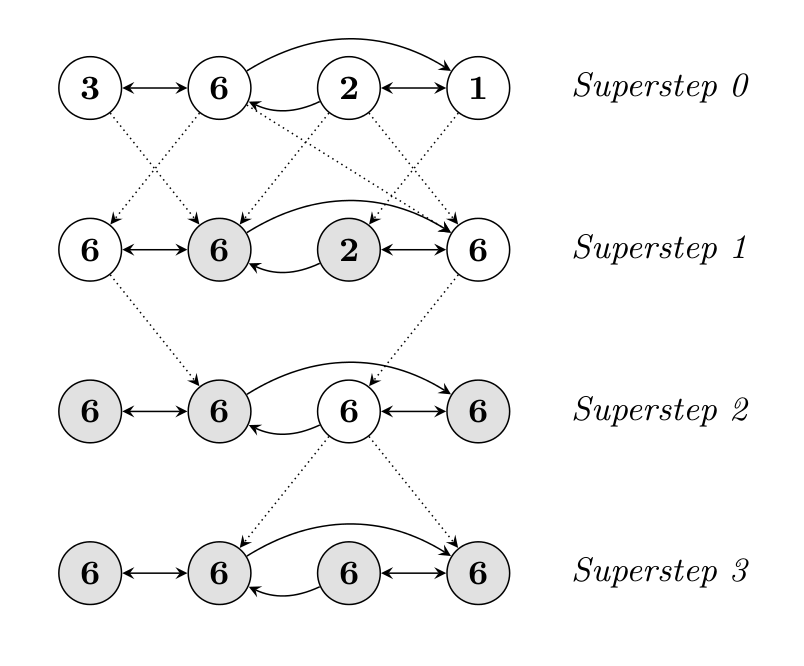
\includegraphics[width=0.6\textwidth]{PregelMaxVal.png}
\caption{Example Pregel computation of maximum value among the nodes. Nodes that voted to halt are marked gray. ()Source: \cite{pregel})}
\end{center}\label{img:pregelmaxval}
\end{figure}

For another example, let us see how single source shortest paths can be computed using Pregel. 
We assume that the value for each vertex is initially set to $\infty$.
In the first superstep the source vertex updates its value to $0$ and sends messages to its neighbors with a new distance. In the following supersteps
other vertices update their distances and send messages to their neighbors with a new possible distance \todo{"wszystkie" -- o co chodzi?}. Each vertex votes to halt in each superstep, so when no more messages with distance updates are sent, the algorithm terminates. This will always happen in a finite number of supersteps, as long as all edges have non-negative lengths. At the end of computation, each vertex has its minimum distance from \textit{SOURCE} associated with it, or $\infty$ if it is not reachable.

\begin{figure}[h!]
\parbox{0.8\textwidth}{
$\text{vertexProgram}(\textit{vertex, superstepNumber, incomingMessages}) \{$

~~~~$\textit{initialDistance} \leftarrow \textbf{if }(vertex.id = SOURCE)~0~\textbf{else}~\infty;$

~~~~$\textit{minDistance} \leftarrow \min(\textit{incomingMessages} \cup \{\textit{initialDistance}\})$;

~~~~\textbf{if} $\textit{newValue} < \textit{vertex.value}$ \textbf{then}

~~~~~~~~$\textit{vertex.value} \leftarrow \textit{minDistance};$

~~~~~~~~\textbf{foreach} $\textit{edge} \in \textit{vertex.outgoingEdges}$ \textbf{do}

~~~~~~~~~~~~~~\text{sendMessage}$(\textit{edge.targetVertex, minDistance + edge.length})$;

~~~~\text{voteToHalt()};

$\}$
}
\todo{lepsze srodowisko do kodu}

\caption{Pregel vertex program for shortest paths from single source to all other vertices}
\end{figure}


An important goal in large dataset computations is to achieve fault-tolerance, so the computation can be continued in case of a failure of some of the machines in the cluster. In Pregel, this is achieved by \emph{checkpointing}. Once in a few supersteps, the workers are required to save their state to the disk. When any of the workers fails, the computation is resumed from the last checkpoint.

In addition to the general model, Pregel also has some additional features enhancing usability and efficiency, such as \emph{aggregators} for efficiently gathering and broadcasting global values and \emph{combiners} which can reduce the network bandwidth used by merging messages send from vertices placed on a given node.

The original implementation by Google engineers is proprietary and was never released to the public. It is written entirely in C++ and tightly connected to the internal Google infrastructure, including the distributed file systems and execution environment.

\section{Giraph}

Giraph \cite{giraph} is an open-source implementation of the Pregel model. It adds several extensions to the version originally described by Google. Those extensions include introducing the possibility to perform computations on the master node, capabilities to work with a support of external memory and removing the single-point-of-failure (SPoF) by adding spare master nodes, which can become active when the primary master node fails.

Giraph is built on top of Hadoop \cite{hadoop}, the widely-adopted framework for large datasets processing. Hadoop is a platform for big datasets computing at scale, consisting of HDFS --- distributed file system, YARN --- framework for managing the cluster and scheduling tasks, Hadoop MapReduce --- an open implementation of the MapReduce model and libraries for using these elements in other projects. \todo{Jak będziesz przerabiał ten rozdział to pewnie to wyląduje gdzie indziej}

Development of Giraph was started by Yahoo!. The project was donated to the Apache Foundation as an incubator project in 2011. It became a Top Level Project of the Apache Foundation in 2012. A stable version 1.0 was released in 2013. There are several large companies including Facebook, Twitter and LinkedIn using the project extensively and engaged in the development. The most active user is Facebook, which executes Giraph programs on social graphs with up to $10^{12} edges$ \cite{giraphfb}. In 2013 Facebook published an article \cite{giraphfb} stating that analyzing so large graphs was impossible with the software available in 2012. The article describes the optimizations and enhancements made in Giraph to be able to run jobs with this amount of data on their infrastructure:
\begin{itemize}
\item Flexible graph input: vertices and edges can be loaded from several sources and the framework takes care of distributing them correctly before the start of computation.
\item Multithreaded execution on a single machine, which allows for better resource sharing than in case of workers distributed across different machines.
\item Memory usage optimization: by serializing the transferred data using primitive types instead of Java objects, the memory usage was significantly reduced, resulting in 10 times lower execution time.
\item Sharded aggregators: instead of aggregators being stored and distributed by the master node, they are stored in a distributed way, which scales better for very large datasets.
\end{itemize}
It is worth mentioning that one of Google Pregel creators and the primary author of the original white paper about it, Grzegorz Malewicz, is one of the members of Facebook's data infrastructure graph processing team which develops Giraph \cite{giraphfb}.

\section{Spark}
Apache Spark \cite{spark, spark2} is an open-source framework for distributed data analytics. It started in 2009 in the AMPLab at University of California, Berkeley. Since that time it has gained a huge momentum and has quickly a growing community of users and contributors \cite{sparkgrowingcommunity}. Since 2009, over 250 individual developers contributed to Spark, and its permanent contributors come from 12 companies and institutions \cite{sparkwww}. Among others, it is being used by companies such as Yahoo, IBM, Intel, Alibaba, Cloudera and Databricks.

Spark's computational model is able to express programs in more specialized models such as MapReduce and Pregel and is also suitable for new applications that these systems do not support, like interactive data mining and stream data processing.

The two key advantages of Spark are:
\begin{itemize}
\item its impressive speed: Spark is in some cases even 100 times faster than equivalent computations in Hadoop MapReduce,
\item its simplicity and ease of use: it offers  APIs in Scala, Java, Python which allow developers to quickly develop programs performing even complicated calculations and a standalone running mode which lets developers set up environment and prototype programs locally without the need to set up Apache Hadoop.
\end{itemize}

Similarly to Apache Giraph, Spark is a Top-Level Project of the Apache Foundation. Previously to promotion as a Top-Level Project in February 2014 \cite{sparktoplevel}, it was in the Apache Incubator program since June 2013. 

Spark fits into the Hadoop ecosystem by being able to run on Hadoop clusters without any additional installation and supporting data input from various Hadoop data stores such as HDFS, HBase and Cassandra. It is not tied, however, to Hadoop infrastructure: it can also run as a standalone deployment in a cluster or on other distributed platforms such as Mesos \cite{mesos} and Amazon EC2 \cite{ec2}.

\subsection{Resilient Distributed Datasets}
The key concept in Spark is the \emph{Resilient Distributed Dataset} (RDD). RDDs are an abstraction of distributed memory, which let the programmer perform distributed computations. They are stored in a way that is transparent to the user and assures fault tolerance.

RDDs provide only a \emph{coarse-grained} interface: operations that are applied to the whole dataset, such as map, filter and join. This allows for achieving fault-tolerance by storing only the history of operations that were used to build a dataset, called its \emph{lineage}, instead of replicating the data to be able to recover it. An additional advantage is that the RDDs do not need to be materialised, unless it is actually necessary. Since parallel computations generally apply some transformation to multiple elements of a dataset, in most cases they can be expressed easily with coarse-grained operation on datasets.

RDDs can be created only in two ways: loading a dataset from a distributed storage or from another dataset by applying coarse-grained functional operations called \emph{transformations}, such as \emph{map}, \emph{filter} and \emph{join}. For greater efficiency, the user can also control the \emph{persistence} by indicating which RDDs are intended to be used in the future and as such should be materialised in the memory and the \emph{partitioning} of each RDD by indicating the key by which the records of RDD should be partitioned across the machines. Finally, the user can perform \emph{actions} on an RDD. Actions return a value or export the dataset to some persistent storage. Avaiable actions include \emph{count}, which returns the number of elements in the RDD, \emph{collect}, which returns the records from the dataset and \emph{save}, which exports the records to an external storage.

\todo{Przykład analogiczny jak dla Pregela i komentarz}

\subsection{Higher level tools}
Spark offers a set of high level tools that demonstrate the capabilities of the Resilient Distributed Dataset model. Those tools are implemented as relatively small libraries on top of Spark's core. Currently available tools are:
\begin{itemize}
\item Spark SQL, allowing seamless integration of SQL queries into Spark programs,
\item Spark Streaming, which supports working on on-line streams of data,
\item MLlib, which is an implementation of common machine learning algorithms for classification, regression, clustering and dimensionality reduction,
\item GraphX, providing an interface for creating efficient graph algorithms, integrated with pre- and post- processing with regular Spark transformations.
\end{itemize}

\section{Other frameworks}
\todo{Opisać krótko GPS, GraphLab, Giraph++. Wspomnieć że są + referencja}





\chapter{SociaLite}\label{r:socialite}

\todo{zastanów się co w jakiej kolejności jest najważniejsze (i zrozumiałe dla czytelnika)}

SociaLite (\cite{socialite, distsoc}) is a graph query language based on Datalog. While Datalog allows to express some of graph algorithms
in an elegant and succinct way, many practical problems cannot be efficiently solved with Datalog programs. 

SociaLite allows a programmer to write intuitive queries using declarative semantics, which can often be executed as efficiently as highly optimized dedicated programs. The queries can then be executed in a distributed environment.

Most significant extension over Datalog in SociaLite is the ability to combine recursive rules with aggregation. Under some conditions, such rules can be evaluated incrementally and thus as efficiently as regular recursion in Datalog.

\cite{socialite} introduces \emph{Sequential SociaLite}, intended to be executed on one machine, consisting of two main extensions: \emph{recursive aggregate functions} and \emph{tail-nested tables}. Recursive aggregate functions are the most important feature in Socialite -- in \ref{s:recaggr} we present a complete definition and proofs of correctness of that extension, which are missing in \cite{socialite}. Tail-nested tables are a much more straightforward extension -- an optimization of data layout in memory. They are described in \ref{s:tnt}

\cite{distsoc} extends Sequential Socialite to \emph{Distributed SociaLite}, executable on a distributed architecture. It introduces a \emph{location operator}, which determines how the data and computations can be distributed. The programmer does not have to think about how to distribute the data between machines or manage the communication between them. He only specifies an abstract \emph{location} for each row in the data, and the data and computations are automatically sharded. Distributed SociaLite is covered in section \ref{s:distributed}

Additionally, thanks to the declarative semantics of Datalog and SociaLite, it is possible to provide an important optimization: the \emph{delta stepping} technique, which is an effective way of parallelizing the Dijkstra algorithm \cite{deltastep}. In SociaLite, this technique can be applied automatically to a certain class of recursive aggregate programs. \todo{zostaw sobie TODO i zastanówi się czy to dasz radę zrobić (potrzebny tu komentarz)
Być może będzie oddzielny rozdział o optymalizacji i te akapity wylądują tam (że oni robili to i to, a ty to i to, bo bardziej pasowało). Wtedy tu wystarczy wspomnieć że w socialite je mają.}

In distributed computations on large graphs, an approximate result is often enough. Usually we can observe the \emph{long tail} phenomenon in the computation, where a good approximate solution is achieved quickly, but it takes a long time to get to the optimal one. In SociaLite, by simply stopping the computation, we can obtain an approximate solution found so far. \cite{distsoc} also shows a method which can significantly reduce memory requirements by storing the intermediate results in an approximate way using Bloom filters. Those topics are covered in section \ref{s:approxdist} \todo{to np. nie będzie jasne dopóki nie wiemy więcej}

\section{Datalog with recursive aggregate functions}\label{s:recaggr}

In this section we introduce the recursive aggregate functions extension from SociaLite. Since the original SociaLite consists of several extensions to Datalog, we will call the language defined here \emph{Datalog with recursive aggregate functions}, abbreviated \datalogra.

\subsection{Motivation}
Most graph algorithms are essentially some kind of iteration or recursive computation. Simple recursion can be expressed easily in Datalog. However, in many problems the computation results are gradually refined in each iteration, until the final result is reached. Examples of such algorithms are the Dijkstra algorithm for single source shortest paths or PageRank. Usually, it is difficult or impossible to express such algorithms in Datalog efficiently, as it would require computing much more intermediate results than it is actually needed to obtain the solution. We will explain that on an example: a simple program that computes shortest paths from a source node.

A straightforward Datalog program for computing single source shortest paths (starting from node $1$) is presented below. Due to limitations of Datalog, this program computes all possible path lengths from node $1$ to other nodes in the first place, and after that for each node the minimal distance is chosen. Not only this approach results in bad performance, but causes the program to execute infinitely if a loop in the graph is reachable from the source node. \todo{czy to jest w Datalogu?
trzeba wyjaśnić że to już jest rozszerzenie a teraz tylko chodzi o sposób wyliczania i zapętlanie}

\dprog{}{
  & \textsc{Path} (t, d) &&  & \assign & && \textsc{Edge} (1, t, d). & \\
  & \textsc{Path} (t, d) &&  & \assign & && \textsc{Path} (s, d_1), \textsc{Edge} (s, t, d_2), d = d_1 + d_2. & \\
  & \textsc{MinPath} (t, \textsc{Min}(d)) &&  & \assign & && \textsc{Path} (t, d). &
}{Datalog query for computing shortest paths from node 1 to other nodes}{ex:ssspdatalog}

\datalogra allows aggregation to be combined with recursion under some conditions. This allows us to write straightforward programs for such problems, which finish execution in finite time and often are much more efficient than Datalog programs. An example \datalogra program that computes single source shortest paths is presented below. The relation $\textsc{Path}$ is declared so that for each \textit{target} the values in \textit{dist} column are aggregated using minimum operator.


\dprog{
  $\textsc{Edge}(\text{int } \textit{src}, \text{int } \textit{sink}, \text{int } \textit{len}) $ \\
  $\textsc{Path}(\text{int } \textit{target}, \text{int } \textit{dist} \text{ aggregate } \textsc{Min}) $
}{
  & \textsc{Path} (1, 0). &&  & & &&  & \\
  & \textsc{Path} (t, d) &&  & \assign & && \textsc{Path} (s, d_1), \textsc{Edge} (s, t, d_2), d = d_1 + d_2. &
}{SociaLite query for computing shortest paths from node 1 to other nodes}{ex:ssspsocialite}

While being very useful, recursive aggregation rules not always have an unambiguous solution. This is the case only under some conditions on the rules and the aggregation function itself.

Typically, Datalog programs semantics is defined using the fixed point of instance inclusion. This requires that the subsequent computation iterations only add tuples to the database instance, but never remove tuples from the instance. This is the reason for which program \ref{ex:ssspdatalog} is inefficient. When recursive aggregate functions are allowed, this is not the case: a tuple in the instance can be replaced with a different one because a new aggregated value appeared. Consequently, in order to define SociaLite programs semantics in terms of fixed point, we need to use a different order on database instances.

First, we will define a meet operation and show the order that it induces. Then we will show that if the aggregation function is a meet operation and corresponding rules are monotone with respect to this induced order, then the result of the program is unambiguously defined. We will also show how it can be computed efficiently.

\subsection{Meet operation and induced ordering}
\begin{defn}
A binary operation is a \emph{meet} operation if it is idempotent, commutative and associative.
\end{defn}
\todo{Maybe remind definitions of semi-lattice and partial order?}

\subsubsection{Order induced by a meet operation}

A meet operation $\sqcap$ defines a semi-lattice: it induces a partial order $\preceq_\sqcap$ over its domain, such that the result of the operation for any two elements is the least upper bound of those elements with respect to $\preceq_\sqcap$

\begin{exmp}
$\max(a, b)$ for $a, b \in \mathbb{N}$ is a meet operation; it is:
\begin{itemize}
\item idempotent -- $\max(a, a) = a$
\item commutative -- $\max(a, b) = \max(b, a)$
\item associative -- $\max(a, \max(b, c)) = \max(\max(a, b), c)$
\end{itemize}
It induces the partial order $\le$: for any two $a, b \in \mathbb{N}$, $\max(a, b)$ is their least upper bound with respect to $\le$.


On the contrary, $+$ is not a meet operation, since it is not idempotent: $1+1 \ne 1$.
\end{exmp}

\subsection{A program in \datalogra}
A \datalogra program is a Datalog program, with additional aggregation function defined for some of the relations:
For each relation $R$, there can be one column $\aggcol_R \in {1, \dots ar_R}$ chosen for which an aggregation function $\aggfun_R$ is provided. The rest of the columns are called the \emph{qualifying columns}. Intuitively, after each step of computation, we group the tuples in the relation by the qualifying columns and aggregate the column $\aggcol_R$ using $\aggfun_R$. Value $\aggcol_R = \bf{none}$ means that $R$ is a regular relation with no aggregation.

For simplicity, we assume that if a relation has an aggregated column, then it is always the last one: $\aggcol_R = ar_R$.

Syntactically, we require that each relation is declared at the top of the program as on the example below. In declaration of a relation, aggregated column can be specified by adding keyword \textit{aggregate} and name of the aggregate function next to the column declaration.

\begin{figure}[h!]
\narrow{
  $\textsc{P}(\text{int } \textit{a}, \text{int } \textit{b} \text{ aggregate } \textsc{F}) $\\
  $\textsc{R}(\text{int } \textit{src}, \text{int } \textit{sink}, \text{int } \textit{len}) $ 
  \begin{flalign*}
  & \textsc{P} (x_1, \dots, x_{ar_P}) &&  & \assign & && Q_{P,1}(x_1, \dots, x_{ar_P}) & \\
  &  &&  & \dots & && & \\
  & \textsc{P} (x_1, \dots, x_{ar_P}) &&  & \assign & && Q_{P,m}(x_1, \dots, x_{ar_P}) & \\
  & \textsc{R} (x_1, \dots, x_{ar_R}) &&  & \assign & && Q_{R,1}(x_1, \dots, x_{ar_R}) & \\
  &  &&  & \dots & && & \\
  & \textsc{R} (x_1, \dots, x_{ar_R}) &&  & \assign & && Q_{R,m}(x_1, \dots, x_{ar_R}) & \\
  \end{flalign*}
  \caption{Structure of a program in \datalogra.}
}
\end{figure}

\subsubsection{Aggregation operation $g_R$}
An important step in the evaluation of a \datalogra program is grouping the tuples in an instance of each relation and performing the aggregation within each group. We can put that into a formal definition as function $g_R$, which takes a relation instance which may contain multiple tuples with the same set of qualifying parameters and performs the aggregation.
\begin{defn}\label{d:aggregationoperationgr}
For a relation $R$ of arity $ar_R = k$, in let us define $g: \bf{dom}^k \to \bf{dom}^k$:
$$
g_R(I) = \begin{cases}
\{(x_1, \dots, x_{k-1}, \aggfun_R(\{y: (x_1, \dots, x_{k-1}, y) \in I\}): (x_1, \dots, x_{k-1}, x_k) \in I\} & \text{if } \aggcol_R \ne \bf{none} \\
I & \text{otherwise}
\end{cases}
$$
\end{defn}

If $R$ has an aggregated column, $g_R$ groups the tuples in relation instance $I$ by qualifying parameters and performs the aggregation using $\aggfun_R$. For non-aggregated relations, $g_R$ is an identity function.

\subsubsection{Order on relation instances}
In Datalog, we can prove that there is a unique least fixed point for any program. The fundamental fact needed for this proof is that during the evaluation of a Datalog program, if the state of a relation is $I_1$ at some point and $I_2$ at some other point, we know that $I_1 \subseteq I_2$. In \datalogra this property no longer holds: a tuple in $I_1$ can be replaced with different tuple with a lower value in the aggregated column. To be able to define semantics of programs in \datalogra using least fixed point, we need to use a custom order on relation instances.

\begin{defn}
Let $R$ be a relation. Let us define comparison $\sqsubseteq_R$ on relation instances as follows:
\begin{align}
I_1 \sqsubseteq_R I_2 \iff \forall_{(q_1, ..., q_{n-1}, v) \in g_R(I_1)} \exists_{(q_1, ..., q_{n-1}, v') \in g_R(I_2)} v \preceq_{\aggfun_R} v' & \text{ if } \aggcol_R \ne \bf{none} \\
I_1 \sqsubseteq_R I_2 \iff \forall_{(q_1, ..., q_n) \in g_R(I_1)} \exists_{(q_1, ..., q_n) \in g_R(I_2)} & otherwise
\end{align}
\end{defn}

\begin{note}
If $R$ does not have an aggregated column, $g_R(I) = I$ for any $I$, so $\sqsubseteq_R$ is simply the inclusion order $\subseteq$. 
\end{note}

\begin{lem}
For any $R$, $\sqsubseteq_R$ is a partial order.
\end{lem}

\emph{Proof:}

If $R$ does not have an aggregated column, $\sqsubseteq_R$ is the same as inclusion order $\subseteq$, which is a partial order.

If $R$ does have an aggregated column, then:

\begin{itemize}
\item $\sqsubseteq_R$ is reflexive: for each $R$, we have that  $\forall_{(q_1, ..., q_{n-1}, v) \in g(R)} \exists_{(q_1, ..., q_{n-1}, v) \in g(R)} v \preceq_{\aggfun_R} v $ because $\preceq_{\aggfun_R}$ is reflexive. Hence, $R \sqsubseteq_R R$.
\item $\sqsubseteq_R$ is antisimmetric \todo{No, it is not antisimmetric, so this is not a partial order --- how to deal with that?}
\item $\sqsubseteq_R$ is transitive: if $A \sqsubseteq_R B$ and $B \sqsubseteq_R  C$, then $\forall_{(q_1, ..., q_{n-1}, a) \in g(A)} \exists_{(q_1, ..., q_{n-1}, b) \in g(B)} a \preceq_{\aggfun_R} b $ and $\forall_{(q_1, ..., q_{n-1}, b) \in g(B)} \exists_{(q_1, ..., q_{n-1}, c) \in g(C)} b \preceq_{\aggfun_R} c$.

$\preceq_{\aggfun_R}$ is transitive, so $\forall_{(q_1, ..., q_{n-1}, a) \in g(A)} \exists_{(q_1, ..., q_{n-1}, c) \in g(C)} a \preceq_{\aggfun_R} c $, which means that $A \sqsubseteq_R C$.
\end{itemize}

\todo{Because of lack of antisimmetry it is only a preorder, not a partial order ---> how to deal with that?}

\todo{dodatkowy komentarz?}

\begin{exmp}
Let $R$ be a relation with arity $3$, with the last column aggregated using meet operation $\max$.
We recall that for $ \max $, $ \preceq_{\max} $ is the usual order $ \le $.
\begin{itemize}
\item $\{(1, 2, 3)\} \sqsubseteq_R \{(1, 2, 5)\}$, because $3 \le 5$
\item $\{(1, 2, 3)\} \sqsubseteq_R \{(1, 2, 5), (1, 7, 2)\}$ , because $3 \le 5$
\item $\{(1, 2, 3), (1, 2, 8)\} \sqsubseteq_R \{(1, 2, 5)\}$ , because $g_R(\{(1, 2, 3), (1, 2, 8)\}) = \{(1,2,3)\}$ and $3 \le 5$
\item $\{(1, 2, 3), (2, 8, 1)\}$ and  $\sqsubseteq_R \{(1, 2, 5), (1, 7, 2)\}$ are not comparable
\item $\emptyset \sqsubseteq_R \{(1, 2, 3)\}$
\end{itemize}
\end{exmp}

We can easily see that for any $R$ an empty relation instance $\emptyset$ is smaller under $\sqsubseteq_R$  than any other relation instance.


\subsection{Semantics and evaluation - one relation case}\label{ss:semeval1rel}
In this section we will show that the semantics of a \datalogra program can be unambiguously defined using least fixed point, as long as it satisfies some conditions. To simplify the reasoning, we will restrict our attention to programs with only one \emph{idb} relation. In the following section we extend the definitions and theorems presented here to the general case of many \emph{idb} relations.

Let $P$ be a \datalogra program, with only one \emph{idb} relation $R$ of arity $k$ in the form of:

\begin{figure}[h!]
\narrow{
%  $\textsc{R}(x_1, \dots, x_{k-1}, x_k [\text{ aggregate } \textsc{F}]) $\\
  \begin{flalign*}
  & \textsc{R} (x_1, \dots, x_k) &&  & \assign & && Q_1(x_1, \dots, x_k) & \\
  &  &&  & \dots & && & \\
  & \textsc{R} (x_1, \dots, x_k) &&  & \assign & && Q_m(x_1, \dots, x_k) & \\
  \end{flalign*}
}
\end{figure}

$Q_1, \dots, Q_m$ are rule bodies with free variables $x_1, \dots, x_k$. They may contain references to any of the \emph{edb} relations, which are constant during the evaluation or to the only \emph{idb} relation, $R$. We denote evaluation of rule body $Q$ in the context of an instance $I$ of the relation $Q$ as $E_I(Q)$.

Since we consider only one relation $R$, we can simplify the notation: let $\sqsubseteq$ denote $\sqsubseteq_R$ and let $g$ denote the aggregation operation $g_R$ for relation $R$, as defined in Definition \ref{d:aggregationoperationgr}.

Let us define $f: \bf{dom}^k \to \bf{dom}^k$ as the function that evaluates the rules $Q_1, ... Q_m$ based on the given instance of the relation $R$ and and returns its input extended with the set of generated tuples:
$$ f(I) = I \cup \bigcup_{i=1..m} E_I(Q_i) $$

Let $h = g \circ f$. 


\begin{thm}
If $f$ is monotone with respect to $\sqsubseteq$, i.e. $R_1 \subseteq R_2 \rightarrow f(R_1) \subseteq f(R_2)$, and there exists $n \ge 0 $, such that $h^n(\emptyset) = h^{n+1}(\emptyset)$, then $R^* = h^n(\emptyset)$ is the least fixed point of $h$, that is:
\begin{enumerate}
\item $R^* = h(R^*)$, i.e. $R^*$ is a fix-point
\item $R^* \sqsubseteq R$ for all $R$ such that $R = h(R)$, i.e. $R^*$ is smaller than any other fix-point
\end{enumerate}
\end{thm}

\emph{Proof:} 

$g$ is monotone with respect to $\sqsubseteq$. Since we assumed that $f$ is monotone with respect to $\sqsubseteq$, $h = g \circ f$ is also monotone with respect to $\sqsubseteq$. 

We know that $\emptyset$ is smaller under $\sqsubseteq$ than any other element.

Let us suppose that $I'$ is any fix-point of $h$.  We know that $\emptyset \sqsubseteq I'$. Applying $h$ to both sides of the inequality $n$ times, we have that $I^* = h^n(\emptyset) \sqsubseteq h^n(I') = I'$, thanks to the monotonicity of $h$ with respect to $\sqsubseteq$. Therefore, the inductive fixed point $I^*$ is the least fixed point of $h$.

In pseudocode, the evaluation algorithm is straightforward:

\begin{figure}[h!]
\narrow{
$I_0 \leftarrow \emptyset$

$i \leftarrow 0$

do

{\addtolength{\leftskip}{5mm}

$i \leftarrow i + 1$

$I_i \leftarrow h(I_{i-1})$

}

while $I_i \ne I_{i-1}$


\caption{Naive evaluation algorithm for \datalogra programs with one \textit{idb} relation.}
}
\end{figure}



\todo{open questions:
\begin{itemize}
\item How we compute recursive functions with non-meet aggregation operators? -- I can forbid that for now...
\end{itemize}
}


\begin{comment}

\subsection{Semi-naive evaluation -- one relation case}
\emph{Semi-naive evaluation} is the most basic optimization used in Datalog. In comes from the following observation: in a Datalog program, if some rule $Q$ produced a tuple $t$ based on database instance $I_i$ in the $i$-th iteration of the naive evaluation algorithm, then this rule with produce this tuple in each subsequent iteration, because $I_j \supseteq I_i$ for $j > i$. The goal of this optimization is to avoid such redundant computation. It is achieved by joining only subgoals in the body of each rule which have at least one new answer produced in the previous iteration.

In this section we give the algorithm for semi-naive evaluation in \datalogra and show that this optimization is valid.

\subsubsection{Algorithm}

\begin{figure}[h!]
\narrow{
$R_0 \leftarrow \emptyset, \Delta_0 \leftarrow \emptyset$

$i \leftarrow 0$

do

{\addtolength{\leftskip}{5mm}

$i \leftarrow i + 1$

$T_i \leftarrow \bigcup_{l=1..n} f(R_{i-1})$

$R_i \leftarrow g_k(T_i \cup R_{i-1})$

$\Delta_k^i \leftarrow R_k^i - R_k^{i-1}$

}

while not for all $k$ $\Delta_k^i = \emptyset$

\caption{Semi-Naive evaluation algorithm for \datalogra programs with one \textit{idb} relation.}
}
\end{figure}

\end{comment}


\subsection{Semantics and evaluation - multiple relations case}
In this section we extend \datalogra semantics from \ref{ss:semeval1rel} to a general case of possibly many \emph{idb} relations.

Let $P$ be a \datalogra program, with $w$ \emph{idb} relations $R_1, R_2, \dots, R_w$ of arities $k_1, k_2, \dots, k_w$ respectively.

\begin{figure}[h!]
\narrow{
%  $\textsc{R}(x_1, \dots, x_{k-1}, x_k [\text{ aggregate } \textsc{F}]) $\\
  \begin{flalign*}
  & \textsc{R$_1$} (x_1, \dots, x_{k_1}) &&  & \assign & && Q_{1,1}(x_1, \dots, x_{k_1}) & \\
  &  &&  & \dots & && & \\
  & \textsc{R$_1$} (x_1, \dots, x_{k_1}) &&  & \assign & && Q_{1,{m_1}}(x_1, \dots, x_{k_1}) & \\
  &  &&  & \dots & && & \\
  & \textsc{R$_w$} (x_1, \dots, x_{k_w}) &&  & \assign & && Q_{w, 1}(x_1, \dots, x_{k_w}) & \\
  &  &&  & \dots & && & \\
  & \textsc{R$_w$} (x_1, \dots, x_{k_w}) &&  & \assign & && Q_{w, {m_w}}(x_1, \dots, x_{k_w}) & \\
  \end{flalign*}
}
\end{figure}

For $i = 1, \dots, w$, $Q_{i,1}, \dots, Q_{i,m}$ are rule bodies with free variables $x_1, \dots, x_{k_w}$. They may contain references to the \emph{idb} relations $R_1, R_2, \dots R_w$ and the \emph{edb} relations, which are constant during the evaluation. We denote evaluation of rule body $Q$ in the context of an instance $I_1, \dots I_w$ of the relation $R_1, \dots, R_w$ as $E_(I_1, \dots, I_w)(Q)$.

For $i = 1, \dots, w$, $Q_{i,1}, \dots, Q_{i,m}$, let us define $f_i: P(\bf{dom}^{k_1}) \times \dots \times P(\bf{dom}^{k_w}) \to P(\bf{dom}^{k_i})$ as the function that evaluates the rules $Q_{i,1}, ... Q_{i, m_w}$ for relation $R_i$ based on the given instances of the relations $R_1, \dots, R_w$:
$$ f_i(I_1, \dots I_w) = I_i \cup \bigcup_{i=1..{m_w}} E_(I_1, \dots, I_w)(Q_i) $$

Let $h_i = g_{R_i} \circ f_i$. Let $h(I_1, \dots, I_w) = (h_1(I_1, \dots, I_w), \dots, h_w(I_1, \dots, I_w))$

Let $\sqsubseteq = \sqsubseteq_{R_1} \times \dots \sqsubseteq_{R_w}$.

\begin{thm}
If $h$ is monotone with respect to $\sqsubseteq$, i.e. $I \subseteq I' \rightarrow h(I) \subseteq f(I')$, and there exists $n \ge 0 $, such that $h^n(\emptyset) = h^{n+1}(\emptyset)$, then $I^* = h^n(\emptyset)$ is the least fixed point of $h$, that is:
\begin{enumerate}
\item $I^* = h(I^*)$, i.e. $I^*$ is a fix-point
\item $I^* \sqsubseteq I$ for all $I$ such that $I = h(I)$, i.e. $I^*$ is smaller than any other fix-point
\end{enumerate}
\todo{Extract the definition of fix-point -- it does not have to be here, but where to put it?}
\end{thm}

\emph{Proof:} 

We know that $\emptyset$ is smaller under $\sqsubseteq$ than any other element.

Let us suppose that $I'$ is any fix-point of $h$.  We know that $\emptyset \sqsubseteq I'$. Applying $h$ to both sides of the inequality $n$ times, we have that $I^* = h^n(\emptyset) \sqsubseteq h^n(I') = I'$, thanks to the monotonicity of $h$ with respect to $\sqsubseteq$. Therefore, the inductive fixed point $I^*$ is the least fixed point of $h$.

In pseudocode, the evaluation algorithm is straightforward:

\begin{figure}[h!]
\narrow{
$I_0 \leftarrow (\emptyset, \dots, \emptyset)$

$i \leftarrow 0$

do

{\addtolength{\leftskip}{5mm}

$i \leftarrow i + 1$

$I_i \leftarrow h(I_{i-1})$

}

while $I_i \ne I_{i-1}$

\caption{Naive evaluation algorithm for \datalogra programs with multiple \textit{idb} relations.}
}
\end{figure}


\todo{open questions:
\begin{itemize}
\item How we compute recursive functions with non-meet aggregation operators? -- I can forbid that for now...
\end{itemize}
}


\subsection{Semi-naive evaluation -- one relation case}
\emph{Semi-naive evaluation} is the most basic optimization used in Datalog evaluation. In comes from the following observation: in a Datalog program, if some rule $Q$ produced a tuple $t$ based on database instance $I_i$ in the $i$-th iteration of the naive evaluation algorithm, then this rule with produce this tuple in each subsequent iteration, because $I_j \supseteq I_i$ for $j > i$. The goal of this optimization is to avoid such redundant computation. It is achieved by joining only subgoals in the body of each rule which have at least one new answer produced in the previous iteration.

This optimization can be applied in \datalogra as well. To achieve this, we need to define function $f$ and the evaluation operation $E_I(Q)$ in a different way.




\subsection{\datalogra with negation}
\todo{Basically we do the same thing as in regular Datalog -- stratification}


\section{Tail-nested tables}\label{s:tnt}
Another important extension in SociaLite are \emph{tail nested tables}, which optimize the memory layout so that it can be accessed in a faster way. While being very useful in practice, this optimization is not crucial for running such programs on distributed architecture. \todo{I don't want to have this in the compiler, but maybe describe here?}

\section{Distributed SociaLite}\label{s:distributed}

\section{Delta stepping in Distributed SociaLite}\label{s:deltastep}

\section{Approximate evaluation in Distributed SociaLite}\label{s:approxdist}








\chapter{\datalogra on Spark}\label{r:implementation}

\datalogra queries that can be executed in a distributed way can prove to be a very useful tool for performing computations on large datasets, especially on graphs. Our goal is to provide an implementation of \datalogra which will be as close as possible to being practically applicable.

To be useful, such solution has to be reliable, provide ways to interact with various distributed storages, ensure proper fault tolerance and little to no additional work to be run on the existing infrastructure.

Distributed Socialite, covered in section \ref{s:distributed}, describes a way of executing Datalog queries with aggregation in a distributed way, by sharding the data based on one of the columns of each relation and contains an independent implementation of the proposed solution. During tests we have found this implementation unreliable and not ready for production use. We propose an alternative approach to distributed \datalogra queries evaluation and present an implementation of the proposed solution.

Instead of developing an independent project, we have chosen to implement \datalogra as an extension to Apache Spark. Thanks to this approach, the implementation can read from and write to all popular Hadoop distributed data stores, including HDFS, HBase and Cassandra \cite{sparkwww}. In can be used on any existing cluster that supports Spark, including Hadoop YARN \cite{hadoop}, Mesos and standalone Spark clusters \cite{sparkwww} and has the industrial-quality fault tolerance and efficiency features developed by hundreds of Apache Spark contributors \cite{githubspark}. 

Using Spark Datalog API, Datalog queries can be integrated seamlessly into Spark programs. One can choose to use Datalog for all computations or only for selected parts of the computation where it serves best. He can also run Datalog queries interactively using the Spark Shell.

In this chapter describe how Datalog and \datalogra queries can be translated into operations allowed in the RDD model. This method was used to implement the  Datalog API for Spark, which enables using Datalog queries in Spark programs. The implementation is evaluated in section \ref{s:impl_eval}.

\section{Integrating Datalog into Spark}

Spark programs describe the computation as a series of calls to functions, which perform one of the following:
\begin{itemize}
  \item create an RDD, generally by reading it from a distributed data source such as HDFS
  \item transform an RDD or several RDDs into another RDD, with methods such as \emph{map}, \emph{filter} or \emph{join},
  \item execute an operation on an RDD, such as storing it HDFS or counting its size.
\end{itemize}

Most of the computation logic is expressed in the transformations.  Core Spark provides only some basic transformations (map, filter, etc todo). Additionally, there are several extensions: GraphX, Spark SQL, MLib. Typically, they extend Spark by providing specialized RDDs and composite data structures and additional transformations for them.

The same approach was chosen for adding the ability of executing Datalog queries. The extension is contained in a module called \emph{Spark Datalog API}. The main component it provides is the \emph{Database} class which contains a set of relations and can be created from regular RDDs. Database objects are equipped with a method \emph{datalog}, which performs a Datalog query on this database. The result of a query is a new Database, from which individual relations can be extracted as RDDs. 

Datalog queries can be applied to any set of input RDDs. The input data can be directly loaded from a distributed storage supported by Spark or computed as a transformation of other RDDs. User first creates relations, declaring their arity, and groups them into a database. Next, he can perform any query on this database, using its \emph{datalog} method. If there are no errors in the query, the result is a new database, containing all computed relations. Each relation can be extracted from the database by giving its name. Figure \ref{sdinspark} shows an example of a \datalogra query used in a Spark program using Datalog API for Spark.

\begin{figure}[h!]
  \centering
\begin{Verbatim}
\textcolor{RedViolet}{val} \textcolor{RoyalPurple}{edgesRdd} = \textcolor{gray}{... // RDD of edge tuples read from disk or computed using Spark}

\textcolor{RedViolet}{val} \textcolor{RoyalPurple}{database} = \textcolor{RoyalPurple}{Database}(\textcolor{RoyalPurple}{Relation}.ternary(\textcolor{BurntOrange}{"Edge"}, edgesRdd))
\textcolor{RedViolet}{val} \textcolor{RoyalPurple}{resultDatabase} = database.datalog(\textcolor{vdarkgray}{"""}
    \textcolor{vdarkgray}{\textcolor{RedViolet}{declare} \textcolor{RoyalPurple}{Path}(int v, int dist \textcolor{RedViolet}{aggregate} Min).}
    \textcolor{vdarkgray}{\textcolor{RoyalPurple}{Path}(x, d) :- s == 1, \textcolor{RoyalPurple}{Edge}(s, x, d).}
    \textcolor{vdarkgray}{\textcolor{RoyalPurple}{Path}(x, d) :- \textcolor{RoyalPurple}{Path}(y, da), \textcolor{RoyalPurple}{Edge}(y, x, db), d = da + db.}
\textcolor{vdarkgray}{"""})
\textcolor{RedViolet}{val} \textcolor{RoyalPurple}{resultPathsRdd} = resultDatabase(\textcolor{BurntOrange}{"Path"})

\textcolor{gray}{... // Save or use resultPathsRdd as any RDD.}
\end{Verbatim}
  \caption{Example of Datalog query for computing single source shortests paths embedded in a Spark program.\label{sdinspark}}
\end{figure}
\section{Executing Datalog queries in the RDD model}

When a Datalog query is performed on the Database object, it needs to be translated into a sequence of Spark transformations which eventually produce a new Database object, containing the result of the query. In this section, we show how this translation can be made.

\subsection{Data representation}

Input and output of Datalog programs is represented as a Database object. Database is simply a set of several Relations.

Each Relation object has a name and an RDD of Facts, which in turn are represented as arrays. All Facts in a relation are required to have the same arity --- this is ensured when the Relation is created.

\emph{Valuation} objects are not available to the end user, but they play significant role during the evaluation. They which represents valuations, which are functions mapping variables to their values. For performance reasons, instead of being represented as a map, they are represented as raw arrays, which layout is determined using the information generated during the analysis phase.

\subsection{Datalog program execution}

On the top level, the algorithm for executing a Datalog program on Spark consists of the following steps:

\begin{enumerate}
\item Analysis phase: Initially, the program is parsed, analyzed syntatically and semantically. All correctness requirements are checked at this time.

\item Stratification: Analyzed program is then stratified, i.e. divided into a sequence of strata using a standard strongly connected components algorithm.

\item Evaluation phase, which starts by evaluating the first stratum of the program on the input database. Each subsequent stratum is then evaluated using the output of the previous stratum as an input. The output of the last stratum is returned as the output of the whole program.

\end{enumerate}

To evaluate each stratum, the semi-naive evaluation algorithm is used. It maintains current state of the database and runs iteratively until no changes are made to the database. In each iteration, for each rule in this stratum, all inferrable facts are computed. The way this can be achieved on RDDs is described in section \ref{ss:impl_evalrule}. The set of obtained facts is then merged into the current database and a \emph{delta}, i.e. difference between current and previous database state is computed. During the merge, all necessary aggregations are applied. This step is described in section \ref{ss:impl_merge}.

\subsection{Single rule evaluation}\label{ss:impl_evalrule}
Evaluation of a single rule plays crucial role in evaluating a Datalog query on RDDs. Given a single rule, consisting of a head and a sequence of subgoals, and two databases: the full input database and the delta database, the task is to compute an RDD of all facts that can be inferred. This is done in two steps: first, all valuations satisfying the rule body are computed, and then each such valuation is converted to a fact based on the head of the rule.

The subgoals are sorted topologically during the analysis phase, so that the evaluation can be performed sequentially, subgoal by subgoal and it is assured that all variables required by the arithmetic subgoals are introduced by an earlier subgoal.

\subsubsection{Evaluating a subgoal on a single valuation}
Let us start from the most basic scenario: evaluating a single relational subgoal $R(x_1, \dots, x_n)$ on a starting valuation $v$, i.e. finding a set of all valuations which satisfy $R(x_1, \dots, x_n)$ and are supersets of $v$. To do this, we can find all facts in the relation $R$ that match $v$ on the \emph{matching variables}, i.e. those which appear both in valuation and in the subgoal. Each such fact yields an extended valuation, consisting of $v$ and valuation for variables from the subgoal.

For example, given a subgoal \relat{Edge}{(v, u, d)} and a valuation $\{v: 5, t: 3\}$, if \textsc{Edge}  contains \relat{Edge}{(5, 1, 2)}, \relat{Edge}{(5, 3, 4)} and \relat{Edge}{(1, 2, 3)}, the result will be $\{\{v: 5, t: 3, u: 1, d: 2\}, \{v: 5, t: 3, u: 3, d: 4\}\}$.

This algorithm could be realised using \emph{map} and \emph{filter} transformations on the relation in the subgoal.

The other types of subgoals are more straightforward. Arithmetic comparison subgoals, e.g. $x < y + z$ are simply evaluated to a boolean value and yield $\{v\}$ if the result was true, and an empty set if the result was not true. In case of assignment subgoals, e.g. $x = y + z$, the expression is evaluated and the corresponding value for the variable is inserted into valuation. If this causes a conflict with a different value for that variable, an empty set is returned. Otherwise, the result is a singleton containing the new variable.

\subsubsection{Evaluating a subgoal on a set of valuations}
During evaluation a sequence of subgoals, instead of having just one starting valuation, we have an RDD of valuations to start with. The result of evaluating a subgoal on an RDD of starting valuations should be the set of all valuations which satisfy the subgoal and are supersets of at least one of the starting valuations. To find it efficiently, the relation is mapped into valuations of the subgoal variables. The resulting RDD is then joined with the starting valuations on the matching variables using the \emph{join} transformation on RDDs.

Arithmetic comparison subgoals are translated into a \emph{filter} transformation on the valuations RDD. They are filtered using a function that checks whether the comparison yields true for that valuation. 

Assignment subgoals are translated into a \emph{map} transformation on the valuations RDD, combined with flattening of the results. For each valuation, the assignment can either be mapped to a singleton or an empty set, so the result of applying this mapping is a RDD of sets, therefore it needs to be flattened so that the result is a plain RDD of valuations.

\subsubsection{Evaluating a sequence of subgoals}
Using the method for evaluating a single subgoal on an RDD of valuations described above, evaluating a sequence of subgoals is straigthforward. 

We start with an RDD of valuations containing an empty valuation, i.e. a valuation which does not contain any variable assignments. Next, we apply subgoals sequentially. Each subgoal is evaluated on the current RDD of valuations. This returns a new RDD of valuations, which all satisfy this subgoal. This new RDD is then used in for the next subgoal, until all subgoals are processed.

\subsubsection{Processing rule head: converting valuations into facts}

Each rule head consists of a relation name and a sequence of variable names, e.g. \relat{Path}{(v, d)}. Language constraints assure that each valuation that satisfies the rule body contains values for all variables appearing in the head, so a fact can be computed from a valuation by looking up corresponding variables in the valuation. Given an RDD of valuations obtained by evaluating the sequence of subgoals in the rule body, this is done by applying a \emph{map} transformation to this RDD.

\subsubsection{Naive and semi-naive evaluation}
If full database is used to retrieve the contents of the relation in each subgoal, the evaluation procedure described in the previous sections will perform naive evaluation.

For the semi-naive evaluation to be performed, the delta database needs to be used. Precisely, the rule body is evaluated separately for each subgoal that uses a relation that is in the \emph{idb} of the current stratum. Contents of the relation for the selected subgoal is retrieved from the delta database and the full database is used in all other subgoals.

\subsection{Adding new facts to database}\label{ss:impl_merge}

The procedure covered in section \ref{ss:impl_evalrule} allows for finding all facts that can be inferred using a single rule. This can be done for each rule within a stratum. The next step in one iteration of evaluation is to merge the results obtained with the existing database.

In case of relations without aggregation, this is achieved by performing the \emph{union} transformation on the RDDs containing new facts for a given relation and the corresponding relation in the current database. It is possible that this introduces duplicated facts, so the \emph{distinct} transformation is used to remove the duplicates.

In case of relations that need to be aggregated, this is slightly different. After performing a union of the new facts and current relation contents, the facts are grouped by the qualifying parameters and the aggregated value is computed by applying the aggregation function. This is done by a sequence of \emph{map} and \emph{reduceByKey} transformations on RDDs.

\subsection{Handling RDD caching, materialization and lineage}
A practial implementation of the evaluation procedure described above requires several RDD-specific issues to be handled:
\begin{itemize}
\item reused RDDs need to be marked to be \emph{cached} in order for them to be stored in memory and not recomputed each time they are used. The databases are marked for caching after each iteration step,
\item results obtained from an iteration and marked to be cached are materialized, i.e. actually computed. This allows for the results of the previous iteration to be \emph{unpersisted}, i.e. removed from cache, as they will no longer be necessary. Unpersisting RDDs helps reduce memory usage and increases performance,
\item if many iterations are performed, the procedure can create RDDs with a very long \emph{lineage}. Lineage is stored in RDDs so that they can be restored after a failure of a worker. Too long lineage can cause errors, so once in every several iterations all results are checkpointed to persistent storage, which causes the lineage to be cropped,
\item most of RDD transformations do not change the partitioning of the data, i.e. the way the data is distributed between worker nodes. However, \emph{join} transformations which are used in the evaluation, increase the number of partitions. Number of partitions too large compared to the size of data can negatively impact performance, so it is reduced when necessary.
\end{itemize}


\subsection{Optimizations}
The main implemented optimization was the semi-naive evaluation. Additionally, several smaller optimizations have been implemented:
\begin{itemize}
\item Non-recursive strata which define only one relation are a common case. In this case, it is clear upfront that one iteration is enough for all facts to be inferred, so the evaluation of the stratum is finished after one iteration instead of performing one more iteration only to notice that there were no changes in the database.
\item Some rule bodies start with subgoals which define constants, e.g. $\textsc{Path}(v,t) :- s~=~1, \textsc{Edge}(s, v, t)$. When subgoals are topologically sorted, such subgoals are placed at the beginning of subgoals sequence. In order for the evaluation of the constant subgoals not to be repeated, the initial sequence of constant subgoals is evaluated during the analysis phase. The result is then used as an initial valuation when evaluating the rest of subgoals in each iteration when this rule body is considered.
\item Within each stratum, necessary \emph{edb} relations are identified and converted to an internal form prepared for futher operations. This allows to avoid repeated work in each of iterations within a stratum, since \emph{edb} relations cannot change.
\end{itemize}

\section{Experiments}\label{s:impl_eval}
Spark Datalog API has been implemented as a fully working prototype. It has been evaluated on clusters of up to 16 Amazon EC2 wroker instances. In this section we provide three sets of experimental results. \datalogra is not limited to a specific domain and can be used to express various types of distributed computations, but it is primarily intended for computations on large graphs such as social networks. Therefore, for performance tests of the prototype implementation, we have selected three common graph problems: 
\begin{itemize}
\item finding and counting triangles: find all triangles in a graph, i.e. triplets of vertices which form a complete graph; additionally, the total count of triangles should be computed,
\item dividing the graph into connected components, i.e. maximal subgraphs in which each pair of vertices is connected by a path,
\item computing shortests paths from a single source to all other vertices.
\end{itemize}

The performance of the tested implementation was compared with plain Spark programs solving the same problem. The plain Spark implementations were written using Spark core methods and the \emph{pregel} operation provided by the GraphX extension. In addition to performance, an interesting property is the complexity of each solution, which can be roughly measured by the number of lines in each program.
% All programs used in the tests are presented in Appedix \todo{ref}.

For each problem, both solutions have been evaluated on Amazon EC2 clusters consisting of 2, 4, 8 and 16 worker nodes and one master node. Each node was a 2-core 64-bit machine with 7.5 GiB of RAM memory.  In all experiments, a social graph of Twitter circles \cite{twitterdata}, which has 2.4M edges was used.

Figure \ref{img_plots_exp} presents the execution times and speedups of SparkDatalog and plain Spark programs for each test case. The SparkDatalog versions are consistently slower than dedicated Spark programs, by a factor approximately 2 in Triangles Counting, 8.5 to 3.5 in Shortest Paths and 4 - 1.7 in Connected Components. The reasons for that are analyzed in section \ref{s:whyslow}. The speedups achieved were similar for both versions of each program. This shows that although the implemented solution is slower by some factor, it does parallelize. In case of Connected Components and Shortest paths, Spark Datalog's speedups were slightly better. This is probably because of the fact that the additional overhead in Spark Datalog execution time over dedicated Spark could also get parallelized. In general, the difference in execution times is the least with the greatest number of worker nodes.

\begin{figure}[h!]
  \centering
    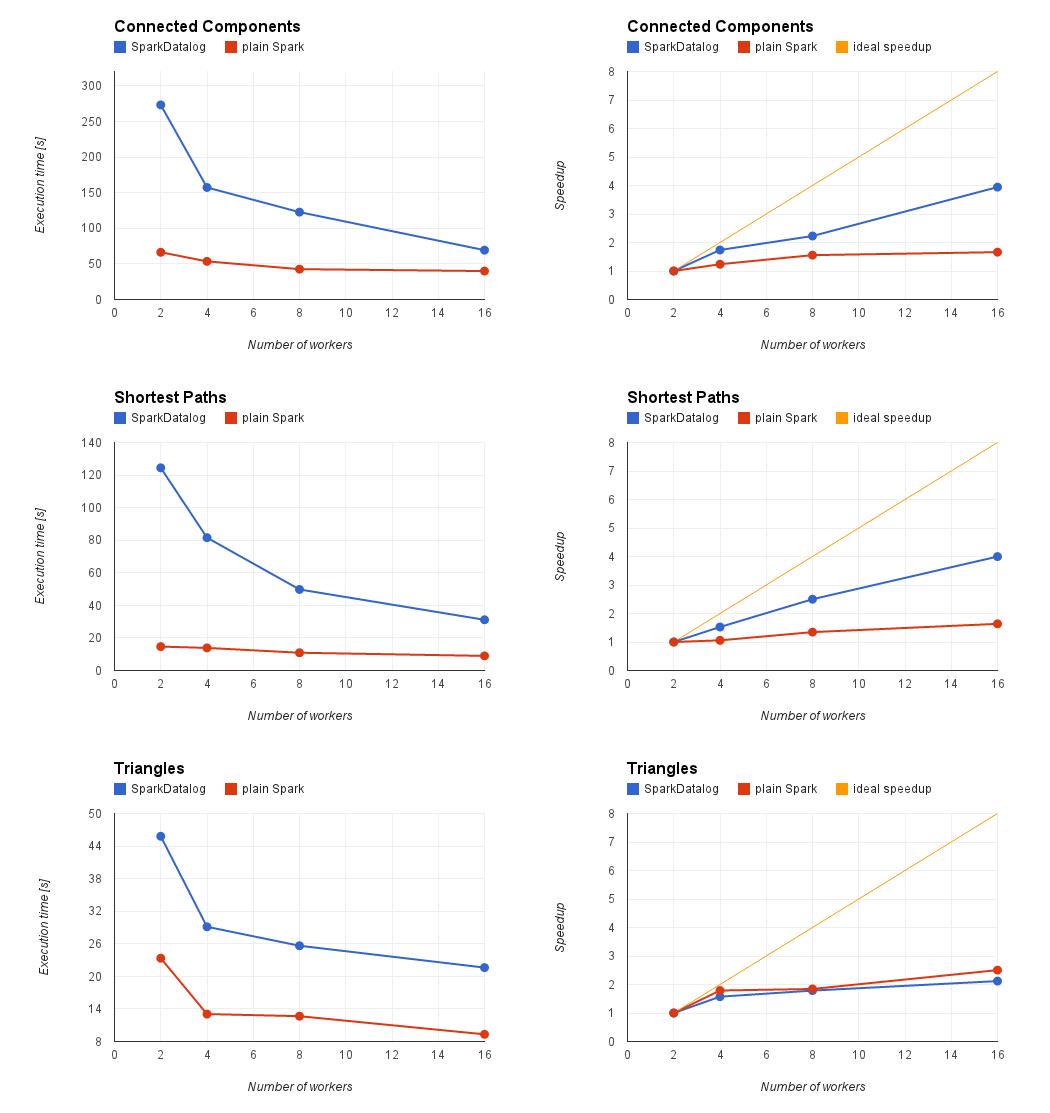
\includegraphics[width=\textwidth]{images/plots_all.png}
   \caption{Results of experiments. \label{img_plots_exp}}
\end{figure}


\begin{table}[h!]
  \centering
\begin{tabular}{l|r|r}
\hline   & plain Spark & SparkDatalog \\ 
\hline
 Connected Components & 13 & 6 \\ 
 Shortest Paths & 14 & 4 \\ 
 Triangles & 7 & 5 \\ 
\hline 
\end{tabular} 
\caption{Number of lines of code in programs, excluding data loading and comments.}
\label{tab_proglen}
\end{table}

An important goal for SparkDatalog is to provide programmers and non-programming analysts with a possibility to perform computations by writing declarative queries instead of implementing complicated, lengthy algorithms using the Pregel model or standard RDD transformations. Table \ref{tab_proglen} shows a comparison of lengths of Spark Datalog and plain Spark programs for each of the problems. Datalog versions are 1.4 to 3.5 shorter than dedicated Spark. Most importantly, they are conceptually simpler, since they only require a few declarative rules, instead of expressing the problem in the vertex-centric Pregel model.

\section{Performance differences}
The SparkDatalog programs are several times slower than their dedicated Spark counterparts. There are several reasons for that, which can be eliminated or minimized in future versions of Spark Datalog:
\begin{enumerate}
\item SparkDatalog uses a general way of conversion of a Datalog program to a sequence of Spark transformations, which results in suboptimal execution of the query, whereas dedicated Spark program executes precisely the necessary operations. This can be resolved or minimized by more work on optimizing the generated execution plan.
\item The internal data representation has a significant impact on the performance. In dedicated Spark programs, native Scala tuples are used. SparkDatalog, on the other hand, currently uses arrays, which are less efficiently serialized and hashed. This results in a significant performance overhead. This could be resolved by representing the most common arities, e.g. 1-5 with tuples and using pre-generated code to work with them.
\item The most costly operation in SparkDatalog execution is repartitioning objects by the hash of their key in order to perform a \emph{join}. The partitioning of the data could be optimized, so that the need to transfer and repartition the data is minimized. This can possibly result in a significant performance gain.
\end{enumerate}

In addition to the above, it is worth adding thanks to the fact that in Datalog problems are expressed in a very high-level, declarative way, it offers very large possibilities of applying optimizations to query execution, for example the \emph{delta-stepping} technique and approximate evaluation \cite{distsoc}. This can result in a significant performance gains over plain Spark programs.


\section{Further work}

There are several areas for further work connected both to the implementation and proposed theoretical solution.

Currently, it is user's responsibility to assure that the program is correct and, in particular, that the rules are monotone with respect to the order implied by the aggregation function used. A theoretical result or an implementation of a tool that helps determine whether the program satisfies this condition is crucial for wide adoption of the proposed language.

Clearly, the performance of the solution is noticeably worse than this of dedicated Spark programs, although the speedups achieved are similar. More work is needed on optimizing the way the queries are executed, including the data representation and partitioning. More sophisticated optimizations of the generated execution, such as elimination of intermediate relations or the \emph{delta-stepping} technique, plan could also be implemented in order to further improve performance.

User experience in embedding the Datalog code in Spark programs could also be improved. Specifically, instead of writing the program as a string, which is then parsed, there could be a domain specific language that would allow for writing similar rules directly in the code. This would allow for type-aware syntax highlighting in IDEs, greater type safety checked at the compile time and additional performace optimizations.






\chapter{Summary}\label{r:summary}





\begin{thebibliography}{99}
\addcontentsline{toc}{chapter}{Bibliography}


\bibitem{socialite} Jiwon Seo, Stephen Guo, Monica S. Lam, \textit{SociaLite: Datalog extensions for efficient social network analysis}, ICDE 2013: 278-289

\bibitem{distsoc} Jiwon Seo, Jongsoo Park, Jaeho Shin, Monica S. Lam: \textit{Distributed SociaLite: A Datalog-Based Language for Large-Scale Graph Analysis}. PVLDB 6(14): 1906-1917 (2013)

\bibitem{fod} S. Abiteboul, R. Hull, and V. Vianu: \textit{Foundations of Databases}. Addison-Wesley (1995)

\bibitem{wfom} T.J. Ameloot, B. Ketsman, F. Neven, D. Zinn: \textit{Weaker Forms of Monotonicity for Declarative Networking: a more fine-grained answer to the CALM-conjecture}, PODS 2014

\bibitem{pagerank} S. Brin, L. Page. \textit{The anatomy of a large-scale hypertextual web search engine.} In WWW’98, 1998.

\bibitem{mapreduce} Jeffrey Dean , Sanjay Ghemawat: \textit{MapReduce: simplified data processing on large clusters}, Proceedings of the 6th conference on Symposium on Opearting Systems Design \& Implementation, 2004

\bibitem{pregel} Grzegorz Malewicz, Matthew H. Austern, Aart J.C. Bik, James C. Dehnert, Ilan Horn, Naty Leiser, Grzegorz Czajkowski: \textit{Pregel: a system for large-scale graph processing}, Proceedings of the 2010 ACM SIGMOD International Conference on Management of data, 2010

\bibitem{giraphpp} Y. Tian, A. Balmin, S. A. Corsten, S. Tatikonda, J. McPherson: \textit{From "Think Like a Vertex" to "Think Like a Graph"}, Proceedings of the VLDB Endowment, 2013

\bibitem{gps}, S. Salihoglun J. Widom: \textit{GPS: A Graph Processing System.} SSDBM, July 2013

\bibitem{deltastep} U. Meyer, P. Sanders: \textit{Delta-stepping: A parallel single source shortest path algorithm.} ESA, 1998.

\bibitem{ullman} Anand Rajaraman, Jeffrey D. Ullman: \textit{Mining of Massive Datasets}, Cambridge University Press, New York, NY, 2011

\bibitem{coddrelmodel} E. F. Codd: \textit{A relational model of data for large shared data banks}, Communications of the ACM, v.13 n.6, 1970

\bibitem{RBS87} R. Ramakrishnan, R. Bancilhon, A. Silberschatz:  \textit{Safety of recursive horn clauses with infinite relations}, Proc. ACM Symp. on Principles of Database Systems, 1987.
\bibitem{KRS88a} M. Kifer, R. Ramakrishnan, A. Silberschatz:  \textit{An axiomatic approach to deciding query safety in deductive databases}, Proc. ACM Symp. on Principles of Database Systems, 1988.
\bibitem{KRS88b} R. Krishnamurthy, R. Ramakrishnan, O. Shmueli:  \textit{A framework for testing safety and effective computability of extended Datalog}, Proc. ACM SIGMOD Symp. on the Management of Data, 1988.
\bibitem{SV89} Y. Sagiv, M. Y. Vardi:  \textit{Safety of datalog queries over infinite databases}.  Proc. ACM Symp. on Principles of Database Systems, 1989.

\bibitem{graphlabwww} http://graphlab.org
\bibitem{graphlab2} Yucheng Low, Joseph Gonzalez, Aapo Kyrola, Danny Bickson, Carlos Guestrin, Joseph M. Hellerstein: \textit{Distributed GraphLab: A Framework for Machine Learning and Data Mining in the Cloud} PVLDB 2012	

\bibitem{graphlab} Yucheng Low, Joseph Gonzalez, Aapo Kyrola, Danny Bickson, Carlos Guestrin, Joseph M. Hellerstein: \textit{GraphLab: A New Parallel Framework for Machine Learning.} Conference on Uncertainty in Artificial Intelligence, 2010.

\bibitem{spark} Matei Zaharia, Mosharaf Chowdhury, Michael J. Franklin, Scott Shenker, Ion Stoica: \textit{Spark: Cluster Computing with Working Sets}, HotCloud 2010
\bibitem{spark2} Matei Zaharia, Mosharaf Chowdhury, Tathagata Das, Ankur Dave, Justin Ma, Murphy McCauley, Michael J. Franklin, Scott Shenker, Ion Stoica: \textit{Resilient distributed datasets: a fault-tolerant abstraction for in-memory cluster computing.} In Proceedings of the 9th USENIX conference on Networked Systems Design and Implementation (NSDI'12), 2012
\bibitem{pointanalysis} J. Whaley, M. S. Lam: \textit{Cloning-based context-sensitive pointer alias analyses using binary decision diagrams} In PLDI, 2004.
\bibitem{boomanalysis} P. Alvaro, T. Condie, N. Conway, K. Elmeleegy, J. M. Hellerstein, R. C. Sears: \textit{Boom analytics: Exploring data-centric, declarative programming for the cloud}, In EuroSys, 2010.
\bibitem{dataloganalysis} P. Alvaro, W. R. Marczak, N. Conway, J. M. Hellerstein, D. Maier, R. Sears. \textit{Dedalus: Datalog in time and space.} In Datalog, 2010

\bibitem{bsp} Leslie G. Valiant, \emph{A Bridging Model for Parallel Computation.} Comm. ACM 33(8), 1990, 103–111.

\bibitem{bgl} Jeremy G. Siek, Lie-Quan Lee, Andrew Lumsdaine: \textit{The Boost Graph Library: User Guide and Reference Manual.} Addison Wesley, 2002.
\bibitem{parallelbgl} Douglas Gregor, Andrew Lumsdaine: \textit{The Parallel BGL: A Generic Library for Distributed Graph Computations.} Proc. of Parallel Object-Oriented Scientific Computing (POOSC), July 2005.
\bibitem{GraphBase} Donald E. Knuth: \textit{Stanford GraphBase: A Platform for Combinatorial Computing.} ACM Press, 1994.

\bibitem{logicblox} http://www.logicblox.com/technology.html, Accessed: September 18th, 2014
\bibitem{datomic} http://www.datomic.com, Accessed: September 18th, 2014
\bibitem{giraph} http://giraph.apache.com, Accessed: September 18th, 2014
\bibitem{sparkwww} http://spark.apache.com, Accessed: September 18th, 2014
\bibitem{hadoop} http://hadoop.apache.com, Accessed: September 18th, 2014
\bibitem{githubspark} https://github.com/apache/spark, Accessed: September 18th, 2014
\bibitem{giraphfb} https://www.facebook.com/notes/facebook-engineering/scaling-apache-giraph-to-a-trillion-edges/10151617006153920, Accessed: September 18th, 2014
\bibitem{sparktoplevel} https://blogs.apache.org/foundation/entry/the\_apache\_software\_foundation\_announces50, Accessed: September 18th, 2014
\bibitem{sparkgrowingcommunity} http://databricks.com/blog/2013/10/27/the-growing-spark-community.html, Accessed: September 18th, 2014
\bibitem{mesos} http://mesos.apache.org, Accessed: September 18th, 2014
\bibitem{ec2} http://aws.amazon.com, Accessed: September 18th, 2014
\bibitem{piglatin} http://pig.apache.org/
\bibitem{hive} http://hive.apache.org/

\bibitem{magicsetsexist} Mario Alviano, Nicola Leone, Marco Manna, Giorgio Terracina, Pierfrancesco Veltri: \textit{Magic-Sets for Datalog with Existential Quantifiers.} Datalog 2012: 31-43
\bibitem{disjunctivedatalog} Mario Alviano, Wolfgang Faber, Nicola Leone, Marco Manna: \textit{Disjunctive datalog with existential quantifiers: Semantics, decidability, and complexity issues.} TPLP 12(4-5): 701-718 (2012)
\bibitem{datalogrelaunched} Francois Bry, Tim Furche, Clemens Ley, Bruno Marnette, Benedikt Linse, Sebastian Schaffert: \textit{Datalog relaunched: simulation unification and value invention}, Proceedings of the First international conference on Datalog Reloaded, March 16-19, 2010, Oxford, UK
\bibitem{magicsets} Francois Bancilhon, David Maier, Yehoshua Sagiv, Jeffrey D Ullman: \textit{Magic sets and other strange ways to implement logic programs}. In Proceedings of the fifth ACM SIGACT-SIGMOD symposium on Principles of database systems (PODS '86). ACM, New York, NY, USA.
\bibitem{subsumptivequeries} K. Tuncay Tekle, Yanhong A. Liu: \textit{More efficient datalog queries: subsumptive tabling beats magic sets.} In Proceedings of the 2011 ACM SIGMOD International Conference on Management of data (SIGMOD '11). ACM, New York, NY, USA.

\bibitem{giraphbook} Claudio Martella, Roman Shaposhnik, Dionysios Logothetis: \textit{Giraph in Action}, Early access edition, http://www.manning.com/martella/

\bibitem{twitterdata} http://snap.stanford.edu/data/egonets-Twitter.html, Accessed: September 18th, 2014 

\end{thebibliography}



%\appendix

%\chapter{Source code of programs used in experiments}\label{appendixa}

\section{Single source shortest paths}
\begin{Verbatim}[label=Shortest paths - SparkDatalog]
val query = """ declare Path(int v, int dist aggregate Min).
                 Path(x, d) :- s == """ + sourceId + """ , Edge(s, x, d).
                 Path(x, d) :- Path(y, da), Edge(y, x, db), d = da + db."""
val resultDatabase = database.datalog(query)
\end{Verbatim}

\vspace{0cm}

\begin{Verbatim}[label=Shortest paths - Spark]
val initialGraph = graph.mapVertices((id, _) => if (id == sourceId) 0.0 else Double.PositiveInfinity)
val sssp = initialGraph.pregel(Double.PositiveInfinity)(
    (id, dist, newDist) => math.min(dist, newDist), // Vertex Program
    triplet => \{  // Send Message
      if (triplet.srcAttr + triplet.attr < triplet.dstAttr) \{
        Iterator((triplet.dstId, triplet.srcAttr + triplet.attr))
      \} else \{
        Iterator.empty
      \}
    \},
    (a,b) => math.min(a,b)) // Merge Message
val shortestPaths = sssp.vertices.map(v => (v._1, v._2))
\end{Verbatim}


\section{Triangles counting}
\begin{Verbatim}[label=Triangles counting - SparkDatalog]
val query = """ |declare Triangle(int v, int w, int u).
                |declare Total(int a, int b aggregate Sum).
                |Triangle(x, y, z) :- Edge(x, y), x < y, Edge (y, z), y < z, Edge(x, z).
                |Total(a, c) :- Triangle(x, y, z), a = 1, c = 1. """.stripMargin
val resultDatabase: Database = database.datalog(query)
\end{Verbatim}

\vspace{0cm}

\begin{Verbatim}[label=Triangles counting - Spark]
val canonicalEdges = edgesRdd.filter(Function.tupled(_ < _)).distinct().cache()
val swappedEdgesRdd = canonicalEdges.map(_.swap)
val pathOf2 = swappedEdgesRdd.join(canonicalEdges).map( \{ case (y, (x, z)) => (x, (y, z)) \} )
val triangle = pathOf2.join(canonicalEdges)
  .filter(\{ case (x, ((y, z), zp)) => z == zp \})
  .map(\{ case (x, ((y, z), zp)) => (x, y, z) \})
val count = triangle.count()
\end{Verbatim}


\section{Connected components}
\begin{Verbatim}[label=Connected components - SparkDatalog]
val query = """ |declare Component(int n, int component aggregate Min).
                |declare ComponentId(int n).
                |Component(n, i) :- Node(n), i = n.
                |Component(n, i) :- Component(p, i), Edge(p, n).
                |ComponentId(id) :- Component(x, id). """.stripMargin
val resultDatabase = database.datalog(query)
\end{Verbatim}

\vspace{0.4cm}

\begin{Verbatim}[label=Connected components - Spark]
val initialGraph = graph.mapVertices((id, _) => id.toInt)
val connectedComponents = initialGraph.pregel(Int.MaxValue)(
  (id, cmp, newCmp) => math.min(cmp, newCmp), // Vertex Program
  triplet => \{  // Send Message
    if (triplet.srcAttr < triplet.dstAttr) \{
      Iterator((triplet.dstId, triplet.srcAttr))
    \} else \{
      Iterator.empty
    \}
  \},
  (a, b) => math.min(a, b)) // Merge Message
\end{Verbatim}

\chapter{Contents of the attached CD}\label{appendixb}

The attached CD contains the implementation of the SparkDatalog extension for Spark described in this thesis and the results of the experiments. The repository containing the implementation is also published at \emph{https://github.com/marekrogala/sparkdatalog}. The CD has the following structure:
\begin{itemize}
\item \emph{implementation/}
	\begin{itemize}
	\item \emph{parsergen/} --- parser generator files,
	\item \emph{sparkdatalog/} --- SparkDatalog extension source code,
	\end{itemize}
\item \emph{experiments/} --- results of experiments,
\item \emph{thesis/} --- this thesis in electronic version.
\end{itemize}


\end{document}

